\documentclass[11pt,          % font size: 11pt or 12pt
               phd,           % degree:    ms or phd
               onehalfspacing % spacing: onehalfspacing or doublespacing
               ]{ncsuthesis}

%%----------------------------------------------------------------------------%%
%%------------------------------ Import Packages -----------------------------%%
%%----------------------------------------------------------------------------%%

\usepackage{ccicons} % creative commons symbols
\usepackage{booktabs}  % professionally typeset tables
\usepackage{amsmath}%,amssymb,amsfonts}
\usepackage{textcomp}  % better copyright sign, among other things
%\usepackage{xcolor}
\usepackage{lipsum}    % filler text
\usepackage[parfill]{parskip}
\usepackage{caption}
\usepackage{subcaption}
\usepackage{paralist}
\usepackage{listings}
\usepackage[inline]{enumitem}
\usepackage[super]{nth}
\usepackage[final]{pdfpages}
\usepackage[final]{pdfpages}

\RequirePackage[
			style=sigchi, %numeric-comp,%authoryear-comp,%trad-abbrv,%nature,
			sorting=nyt,%ynt					
			hyperref=true, %	
			firstinits=true,%
			backend=bibtex, %biber
			natbib=true,
			url=false,
			isbn=false,
			maxnames=2, %for et al to be used
			maxalphanames=1, %to avoid printing a + for every et al in the abbreviation
			doi=true]{biblatex}		

% ------------------------------ Bibliography -----------------------------

%needed to do et al after two names
%http://tex.stackexchange.com/questions/44048/use-et-al-in-biblatex-custom-style
\renewcommand*{\finalnamedelim}{\addspace\&\space}

%Simplify abbreviation (the default uses either one or two authors and it indicates et al with a +)
%The following five lines make it so that only the first author is used in the abbreviation
%http://tex.stackexchange.com/questions/27956/label-only-from-first-author
\renewcommand*{\labelalphaothers}{}
    \renewcommand*{\intitlepunct}{}
    \DefineBibliographyStrings{german}{in={}}
    \DefineBibliographyStrings{english}{in={}}
    \DeclareNameAlias{sortname}{last-first}
    \DeclareNameAlias{default}{last-first}
	
%\AtEveryCitekey{\ifciteseen{}{\defcounter{maxnames}{99}}} %authoryear			
\DeclareFieldFormat[article,periodical]{volume}{\mkbibbold{#1}}
\makeatletter

\newrobustcmd*{\parentexttrack}[1]{%
  \begingroup
  \blx@blxinit
  \blx@setsfcodes
  \blx@bibopenparen#1\blx@bibcloseparen
  \endgroup}

\AtEveryCite{%
  \let\parentext=\parentexttrack%
  \let\bibopenparen=\bibopenbracket%
  \let\bibcloseparen=\bibclosebracket}

\makeatother
\renewcommand{\cite}[1]{\parencite{#1}}


\renewbibmacro{in:}{%
  \ifentrytype{article}{}{%
  \printtext{\bibstring{in}\intitlepunct}}}
  
\AtEveryBibitem{\clearfield{month}}

\AtEveryBibitem{\clearfield{language}}

\addbibresource{baharmon-thesis.bib}

 \defbibheading{myheading}[BIBLIOGRAPHY]{
 \chapter*{#1}
 %\centerline{\bf{#1}}
 \markboth{#1}{#1}}

%% FOR TESTING
%\usepackage{showframe}

%\usepackage{amsmath,amssymb,amsfonts} %amssymb and amsfonts cannot be used in conjunction with mdput
%\usepackage{graphicx,subfig}% Include figure files
\usepackage{dcolumn}% Align table columns on decimal point
\usepackage{bm}% bold math
%\usepackage{hyperref}% add hypertext capabilities
%\usepackage{hypernat}% make hyperref and natbib work together
\usepackage{cancel}
\usepackage{verbatim}% multiline commenting
\usepackage{ifthen}
\usepackage{url}
\usepackage{sectsty}
\usepackage{balance} 
%\usepackage{caption}
\usepackage{graphicx} %eps figures can be used instead
\usepackage{lastpage}
\usepackage[format=plain,justification=RaggedRight,singlelinecheck=false,font=small,labelfont=bf,labelsep=space]{caption} 
\usepackage{fancyhdr}
\pagestyle{fancy}
\usepackage{minitoc}
%\usepackage{bibentry}
%\nobibliography*

%http://tex.stackexchange.com/questions/100817/error-when-using-bc-from-abbrevs-in-caption
%Getting BC
\usepackage{abbrevs}
\usepackage{etoolbox}
\robustify{\DateMark} % after having loaded abbrevs

\usepackage{units} %Needed to solve bug from citation Hydrodynamics in 21/2 dimensions
%see http://www.latex-community.org/viewtopic.php?f=5&t=989

\usepackage[sharp]{easylist} %used for brainstorming purposes 
%\usepackage{mathabx} % used for \Asterisk for convolution %conflicts with \widering

%compile on single pass
%\usepackage[backend=biber]{biblatex}


%%%%%%%%%%%%
%%% Hack to make chapters start on odd pages
% http://tex.stackexchange.com/questions/73591/how-to-have-a-blank-even-page-before-every-chapter
%%%%%%%%%%%%
%\newcommand{\ensureoddstart}{\checkoddpage\ifoddpage\else\newpage\mbox{}\fi}
%\newcommand{\ensureoddstart}{}


%%%Fancy tables
%http://tex.stackexchange.com/questions/94032/fancy-tables-in-latex
%\usepackage[table]{xcolor}
%\usepackage{array,booktabs}
%\usepackage{colortbl}
%\newcolumntype{L}{@{}>{\kern\tabcolsep}l<{\kern\tabcolsep}}



%%%%%%%%%%
%%%%% Hack to allow more levels in outline
%%%%%%%%%%
%\setcounter{secnumdepth}{5}
%\setcounter{tocdepth}{5} %may violate ETD
%Usage http://pleasemakeanote.blogspot.com/2010/06/how-to-activate-subsubsubsection-in.html
%\section{} % level 1
%\subsection{} % level 2
%\subsubsection{} % level 3
%\paragraph{} % level 4 - equivalent to subsubsubsection
%\subparagraph{} % level 5

%http://tex.stackexchange.com/questions/60209/how-to-add-an-extra-level-of-sections-with-headings-below-subsubsection
\usepackage{titlesec}

\setcounter{secnumdepth}{4}

\titleformat{\paragraph}
{\normalfont\normalsize\bfseries}{\theparagraph}{1em}{}
\titlespacing*{\paragraph}
{0pt}{3.25ex plus 1ex minus .2ex}{1.5ex plus .2ex}

%%%%%%%%%%%%%%%%%%%%%%%%%%
%%%% Hack for containing figures within sections
%%%%%%%%%%%%%%%%%%%%%%%%%%%%
%http://ctan.org/pkg/placeins
\usepackage{placeins}
%De­fines a \FloatBar­rier com­mand, be­yond which floats may not pass; use­ful, for ex­am­ple, to en­sure all floats for a sec­tion ap­pear be­fore the next \sec­tion com­mand.

%%%Hack for centering all figures
%\makeatletter
%\g@addto@macro\@floatboxreset\centering
%\makeatother

%%----------------------------------------------------------------------------%%
%%---------------------------- Formatting Options ----------------------------%%
%%----------------------------------------------------------------------------%%
%%

%% -------------------------------------------------------------------------- %%
%% Disposition format -- any titles, headings, section titles
%%  These formatting commands affect all headings, titles, headings,
%%  so sizing commands should not be used here.
%%  Formatting options to consider are
%%     +  \sffamily - sans serif fonts.  Dispositions are often typeset in
%%                    sans serif, so this is a good option. 
%%     +  \rmfamily - serif fonts
%%     +  \bfseries - bold face
%\dispositionformat{\sffamily\bfseries}   % bold and sans serif
\dispositionformat{\bfseries}            % bold and serif

%% -------------------------------------------------------------------------- %%
%% Formatting for centered headings - Abstract, Dedication, etc. headings
%%  This is where one might put a sizing command.
%%  \MakeUppercase can be used to typeset all headings in uppercase.
\headingformat{\large\MakeUppercase}   % All letters uppercase
%\headingformat{\large}                % Not all uppercase
%\headingformat{\Large\scshape}        % Small Caps, used with serif fonts.

%% Typographers recommend using a normal inter-word space after
%% sentences. TeX's default is to add an wider space, but \frenchspacing
%% gives a normal spacing. Comment out the following line if you prefer
%% wider spaces between sentences.
\frenchspacing


%% -------------------------------------------------------------------------- %%
%%  Optional packages
%%    A number of compatible packages to improve the look and feel of
%%    your document are available in the file optional.tex 
%%    (For example, hyperlinks, fancy chapter headings, and fonts)
%% To use these options, uncomment the next line and see optional.tex
%%  Optional Packages to consider.   These packages are compatible with
%%    ncsuthesis.  

%% -------------------------------------------------------------------------- %%
%% Fancy chapter headings
%%  available options: Sonny, Lenny, Glenn, Conny, Rejne, Bjarne
%\usepackage[Sonny]{fncychap}
%\usepackage[Lenny]{fncychap}
%\usepackage[Glenn]{fncychap}
%\usepackage[Conny]{fncychap}
%\usepackage[Rejne]{fncychap}
%\usepackage[Bjarne]{fncychap}

%% -------------------------------------------------------------------------- %%
%% Chapter headings

\makeatletter
\def\thickhrulefill{\leavevmode \leaders \hrule height 1ex \hfill \kern \z@}
\def\@makechapterhead#1{%
  \vspace*{10\p@}%
  {\parindent \z@ 
        \raggedleft
        \reset@font\Large\bfseries
        \begin{tabular}{c|p{15cm}}
          {\qquad\thechapter{}\  }
          &\quad
          \large #1
        \end{tabular}
        \par\nobreak
    \vskip 100\p@
  }}
\def\@makeschapterhead#1{%
  \vspace*{10\p@}%
  {\parindent \z@ 
        \raggedleft
        \reset@font\Large\bfseries
        \begin{tabular}{cp{15cm}}
          {\qquad\hphantom{\thechapter{}}\  }
          &\quad
          \Large #1
        \end{tabular}
        \par\nobreak
    \vskip 100\p@
  }}


%% -------------------------------------------------------------------------- %%
%% Chapter headings

%\usepackage{titlesec}
%\titleformat{\chapter}[display]
%  {\normalfont\Large\raggedleft}
%  {\MakeUppercase{\chaptertitlename}~%
%    \rlap{ \resizebox{!}{1.5cm}{\thechapter}\rule{6cm}{1.5cm}}}
%  {10pt}{\Large}
%\titlespacing*{\chapter}{0pt}{30pt}{20pt}


%%----------------------------------------------------------------------------%%
%% Hyperref package creates PDF metadata and hyperlinks in Table of Contents
%%  and citations.  Based on feedback from the NCSU thesis editor, 
%%  the links are not visually distinct from normal text (i.e. no change
%%  in color or extra boxes).
\usepackage[
  pdfauthor={Brendan Alexander Harmon},
  pdftitle={Tangible Landscape},
  pdfcreator={pdftex},
  pdfsubject={NC State ETD Thesis},
  pdfkeywords={tangible interfaces, geospatial modeling, geographic information systems, embodied cognition, spatial thinking},
  colorlinks=true,
  linkcolor=black,
  citecolor=black,
  filecolor=black,
  urlcolor=black,
]{hyperref}


%% -------------------------------------------------------------------------- %%
%% Microtype - If you use pdfTeX to compile your thesis, you can use
%%              the microtype package to access advanced typographic
%%              features.  By default, using the microtype package enables
%%              character protrusion (placing glyphs a hair past the right 
%%              margin to make a visually straighter edge)
%%              and font expansion (adjusting font width slightly to get 
%%              more favorable justification).
%%              Using microtype should decrease the number of lines
%%              ending in hyphens.
\usepackage{microtype}


% ------------------------------ Typeface -----------------------------
\usepackage{ifxetex}
\ifxetex
  \usepackage{fontspec}
  \defaultfontfeatures{Ligatures=TeX} % To support LaTeX quoting style
  \setmainfont[Mapping=tex-text, Color=textcolor]{HelveticaNeue}
  %\setmainfont[Mapping=tex-text, Color=textcolor]{Avenir LT Std}
\else
  \usepackage[T1]{fontenc}
  \usepackage[utf8]{inputenc}
  \renewcommand{\familydefault}{\sfdefault}
  \usepackage{helvet}
\fi
\chapterfont{\Large} % \sffamily

%%----------------------------------------------------------------------------%%
%% Fonts 

%% ETD guidelines don't specify the font.  You can enable the fonts
%%  by uncommenting the appropriate lines.  Using the default Computer 
%%  Modern fonts is *not* required.  A few common choices are below.
%%  See http://www.tug.dk/FontCatalogue/ for more options.

%% Serif Fonts -------------------------------------------------
%%  The four serif fonts listed here (Utopia, Palatino, Kerkis,
%%  and Times) all have math support.


%% Utopia
%\usepackage[T1]{fontenc}
%\usepackage[adobe-utopia]{mathdesign}

%% Palatino
%\usepackage[T1]{fontenc}
%\usepackage[sc]{mathpazo}
%\linespread{1.05}

%% Kerkis
%\usepackage[T1]{fontenc}
%\usepackage{kmath,kerkis}

%% Times
%\usepackage[T1]{fontenc}
%\usepackage{mathptmx}


%% Sans serif fonts -------------------------

%\usepackage[scaled]{helvet}  % Helvetica
%\usepackage[scaled]{berasans} % Bera Sans

%solve bug from fancyhdr in optional
%http://nw360.blogspot.com/2006/11/latex-headheight-is-too-small.html
\setlength{\headheight}{14pt}

%%----------------------------------------------------------------------------%%
%%---------------------------- Content Options -------------------------------%%
%%----------------------------------------------------------------------------%%
%% Size of committee: 3, 4, 5, or 6 -- this number includes the chair
\committeesize{4}

%% Members of committee
%%  Each of the following member commands takes an optional argument
%%   to specify their role on the committee.
%%  For co-chairs, use the commands:
%%      \cochairI{Doug Dodd}
%%      \cochairII{Chris Cox}
%%
\cochairI{Eugene Bressler}
\cochairII{Ross Meentemeyer}
\memberI{Art Rice}
\memberII{Helena Mitasova}

%% Student writing thesis, \student{First Middle}{Last}
\student{Brendan Alexander}{Harmon} % a full middle name

%% Degree program
\program{Design}

%% Thesis Title
%%  Keep in mind, according to ETD guidelines:
%%    +  Capitalize first letter of important words.
%%    +  Use inverted pyramid shape if title spans more than one line.
%%
%%  Note: To break the title onto multiple lines, use \break instead of \\.
%\thesistitle{A North Carolina State University Sample \LaTeX{} Thesis \break 
%with a Title So Long it Needs a Line Break}
\thesistitle{Tangible Landscape}

%% Degree year.  Necessary if your degree year doesn't equal the current year.
%\degreeyear{1995}


%%----------------------------------------------------------------------------%%
%%---------------------------- Personal Macros -------------------------------%%
%%----------------------------------------------------------------------------%%

%% A central location to add your favorite macros.

%% A few examples to get you started.
\newcommand{\uv}[1]{\ensuremath{\mathbf{\hat{#1}}}}
\newcommand{\bo}{\ensuremath{\mathbf{\Omega}}}
\newcommand{\eref}[1]{Eq.~\ref{#1}}
\newcommand{\fref}[1]{Fig.~\ref{#1}}
\newcommand{\tref}[1]{Table~\ref{#1}}
\newcommand{\del}{\nabla}
\renewcommand{\exp}[1]{e^{#1}}
\newcommand{\Conv}{\mathop{\scalebox{1.5}{\raisebox{-0.2ex}{$\ast$}}}}%


\usepackage{color}
%\newcommand{\NEW}[1]{\textcolor{blue}{#1}}
\newcommand{\NEW}[1]{#1}
\newcommand{\COMMENT}[1]{\textcolor{green}{#1}}


\newcommand{\NOTER}[1]{\textcolor{orange}{#1}}
\newcommand{\NOTEC}[1]{\textcolor{blue}{#1}}
\newcommand{\NOTEK}[1]{\textcolor{magenta}{#1}}

\newcommand{\mum}{\ensuremath{{\mu}\text{m}}}

%This makes it so that you can add short paths in your .tex by including the folders where you store your images in the search path
\graphicspath{{./Chapter-1/figs/}{./Chapter-2/figs/}{./Chapter-3/figs/}{./Chapter-4/figs/}{./Chapter-5/figs/}}


%%---------------------------------------------------------------------------%%
\usepackage{calc}
%% Capital letter height
\newlength{\chaptercapitalheight}
\settoheight{\chaptercapitalheight}{D}
\newlength{\chapterfootskip}
\setlength{\chapterfootskip}{\chaptercapitalheight}
\addtolength{\chapterfootskip}{2\baselineskip}
\addtolength{\chapterfootskip}{0.5ex}  % A little extra space to ensure there are 2 full double spaced lines
%\def\chapterfootskipnum{\chapterfootskip}
\renewcommand{\listfigurename}{LIST OF FIGURES}
\renewcommand{\listtablename}{LIST OF TABLES}
\renewcommand{\bibname}{BIBLIOGRAPHY}

%\renewcommand{\cfttoctitlefont}{\centering\ncsu@headingformat}


%http://tex.stackexchange.com/questions/47184/height-of-figure-caption-textheight
\newlength\graphht
\newcommand\calculategraphicstargetheight[1]{%
     \setlength\graphht{\textheight 
                       -\parskip
                       -\abovecaptionskip -\belowcaptionskip
                       -(12pt * #1) % assuming baselineskip of 12pt in caption
                       -\chapterfootskip
                       }}

%\usepackage{titlesec}

%landscape support in fancyhdr from http://tex.stackexchange.com/questions/9071/how-to-translate-and-rotate-the-heading-of-landscaped-pages
\usepackage{pdflscape}
\usepackage{tikz}
\fancypagestyle{lscapedplain}{%
  \fancyhf{}
  \fancyfoot{%
    \tikz[remember picture,overlay]
      \node[outer sep=1cm,above,rotate=90] at (current page.east) {\thepage};}
\renewcommand{\headrulewidth}{0pt} 
\renewcommand{\footrulewidth}{0pt}
}
                      
\begin{document}
\pagestyle{plain}

%%---------------------------------------------------------------------------%%
\frontmatter

%% ------------------------------ Abstract ---------------------------------- %%
\begin{abstract}

Tangible interfaces enable users to 
kinaesthetically interact with computations. 
%
Theoretically this should embody cognition in 
human-computer interaction 
so that users can 
cognitively grasp digital data with their bodies and
offload challenging cognitive tasks onto their bodies.
%
I have co-designed Tangible Landscape --
a tangible interface 
powered by a geographic information system --
and used it to study how
tangible computing mediates spatial thinking.

Tangible Landscape
couples a malleable, interactive physical model 
of a landscape with a digital model of the landscape 
so that users can 3D sketch ideas 
and immediately analyze 
them with scientific rigor. 
The physical and digital models are linked through 
a real-time cycle of 
physical interaction, 3D scanning, geospatial computation, and projection. 
As users interact with a physical model of a landscape -- 
for example by sculpting the topography -- 
the changes are scanned into 
a
%GRASS GIS, an open source 
geographic information system (GIS), 
for geospatial analysis and simulation 
and the resulting analytics are projected onto the physical model. 
%
% applications
My colleagues and I have developed applications 
for Tangible Landscape including 
stormwater management, flood control, 
landscape management and erosion control, 
trail planning, viewshed analysis, solar analysis, wildfire management, 
disease spread management, invasive species management, 
urban growth, and sea level rise adaption.

% experiment
In a series of terrain modeling experiments
my colleagues and I studied how Tangible Landscape 
mediates spatial thinking and performance. 
We used quantitive and qualitative methods to assess 
participants' spatial performance 
using digital and tangible modeling. 
We used geospatial analytics 
such as geomorphometry and per-cell statistics
supplemented by semi-structured interviews and direct observation
to analyze multidimensional spatial performance. 
% findings
We found that 3D sketching with Tangible Landscape 
improves 3D % multidimensional 
spatial performance
and enables a rapid iterative modeling process. 
%Users can intuitively interact 
%with multidimensional data and scientific models
%with Tangible Landscape. 
\end{abstract}


%% ---------------------------- Copyright page ------------------------------ %%
%% Comment the next line if you don't want the copyright page included.
\makecopyrightpage

%% -------------------------------- Title page ------------------------------ %%
\maketitlepage

%% -------------------------------- Dedication ------------------------------ %%
%\begin{dedication}
% \centering To my parents.
%\end{dedication}

%% -------------------------------- Biography ------------------------------- %%
\begin{biography}
Brendan is a PhD candidate at North Carolina State University with
a Bachelor of Arts from Sewanee, the University of the South,
a Master of Landscape Architecture from the Harvard Graduate School of Design,
and
a Master of Philosophy in Geography and the Environment from the University of Oxford.
\end{biography}

% ADD A PICTURE

%% ----------------------------- Acknowledgements --------------------------- %%
%\begin{acknowledgements}
%I would like to thank my advisor for his help.
%\end{acknowledgements}


\thesistableofcontents

\thesislistoftables

\thesislistoffigures


%%---------------------------------------------------------------------------%%
\mainmatter

%\pagestyle{fancy}
\pagestyle{plain}

\newgeometry{margin=1in, lmargin=1.25in, footskip=\chapterfootskip, includehead, includefoot}

\includepdfset{
%frame={true},
pagecommand={}
}

\chapter{Introduction}
\label{chap-one}

\section{Tangible interaction}

In a seminal paper Ishii and Ullmer 
envisioned tangible user interfaces that would 
`bridge the gap between cyberspace and the physical environment 
by making digital information (bits) tangible' \cite{Ishii1997}.
They described `tangible bits' as 
`the coupling of bits with graspable physical objects' \cite{Ishii1997}. 
Tangible interfaces 
-- interfaces that couple physical and digital data \cite{Dourish2001} -- 
are designed to physically manifest digital data 
so that users can cognitively grasp and absorb it,
so that we can think with it rather than about it \cite{Kirsh2013}. 
%With a tangible interface both input and output are physical;
%this enables users to
%`take advantage of natural physical affordances 
%to achieve a heightened legibility and seamlessness of interaction 
%between people and information' \cite{Ishii1997}. 
Since 
`the physical state of tangibles 
embodies key aspects of the digital state 
of an underlying computation' \citep{Ishii2008}
data is not just visualized, 
but can also be felt and directly, physically manipulated, 
leveraging highly developed motor skills. 
When interactions are embodied 
intention, action, and feedback 
should be seamlessly connected.
Interaction should be automatic, subconscious, and intuitive.

\section{Tangible geospatial interaction}

Scientific computing can used to study and 
solve complex spatial problems. 
It can be challenging, however, 
to visualize and interact with complex spatial computations.
Tangible interfaces for geospatial modeling 
give spatial computations 
an interactive, physical form
that can be kinaesthetically 
explored and transformed.
Users should be able to 
intuitively grasp, understand, and manipulate 
spatial computations.
These tangible interfaces
should computationally augment users' spatial cognition, 
while offloading the cognitive tasks of 
interaction and perception onto their bodies. 

\subsection{Theory}
%
Theoretically tangible interfaces for geospatial modeling
should enable 
intuitive digital sculpting, 
streamline design processes by seamlessly integrating 
analog and digital workflows, and 
improve collaboration and communication by enabling multiple users 
to simultaneously interact 
in a natural way \cite{Ratti2004}. 
GIS provide the extensive libraries for geospatial databasing, 
processing, analysis, modeling, simulation, and visualization 
needed to address real world problems \cite{Tateosian2010}. 
%
Tangible interfaces for geospatial modeling 
have the potential to make spatial science more intuitive 
by enabling a rapid iterative process 
of observation, hypothesizing, testing, and inference.
With these systems users can for example 
dynamically explore how topographic form 
influences landscape processes \cite{Mitasova2006}. 

% review
A review of tangible interfaces for geospatial modeling
(Tables~\ref{tt-tab-1}-\ref{tt-tab-4}), however, 
reveals a dearth of critical research.
While many prototypes have been developed
there have been 
few case studies or qualitative user studies
and no quantitative studies.
The theories that have inspired 
 tangible interfaces for geospatial modeling
have not yet been critiqued or proven. 

\subsection{Prototypes}

Tangible interfaces like 
Urp \cite{Underkoffler1999}, 
Illuminating Clay \cite{Piper2002a}, 
and SandScape \cite{Ratti2004} 
enriched physical models of urban spaces and landscapes 
with spatial analyses and simulations 
like wind direction, cast shadow, 
slope, aspect, curvature, and water direction
in order to enhance and streamline design processes. 
Many of the analyses used in Illuminating Clay 
were adapted from GRASS GIS \cite{Piper2002a}
and eventually 
Illuminating Clay was coupled with GRASS GIS 
to draw on its extensive libraries for spatial computation. 
The aim of coupling Illuminating Clay with GRASS GIS was to 
`explore relationships that occur between different terrains, 
the physical parameters of terrains, 
and the landscape processes 
that occur in these terrains' \cite{Mitasova2006}. 
The research to couple a physical landscape model with GRASS GIS 
led to the development of 
the Tangible Geospatial Modeling System \cite{Tateosian2010} 
and Tangible Landscape \cite{Petrasova2014,Petrasova2015}.
Tangible Landscape couples a malleable physical model 
and a digital geospatial model of a landscape 
through a real-time cycle of physical interaction, 3D sensing, 
geospatial computation, and projection. 
Tangible Landscape was designed for
natural and collaborative interaction with GIS.
Such natural interaction with geospatial models should 
enhance spatial cognition and encourage spatial learning. 

\section{Research}

%\subsection{Aims and objectives}

% aim
The aim of this research was to make
scientific spatial computing 
natural, rapid, and collaborative
% motivation
in order to
streamline spatial science and design. 
% objective
The objective was to 
design a tangible interface for geospatial modeling
and study how it mediates spatial cognition
in order 
to implement, study, critique, and refine 
theories about tangibles and spatial thinking. 
% questions
Through an iterative cycle of design and research 
my colleagues and I addressed the following research questions: 
\begin{itemize}
\item How can we design an effective tangible interface for geospatial modeling?
\item How can we use tangible geospatial analytics to solve spatial problems?
\item How does coupling physical and digital models of topography mediate spatial thinking?
\item How do different tangible geospatial analytics mediate spatial thinking?
\item How do tangible geospatial analytics
mediate how users relate form and process?
\end{itemize}

\subsection{Methods}
%In an iterative cycle of design and research
I co-designed Tangible Landscape 
and ran a series of terrain modeling experiments 
studying how tangible geospatial modeling 
mediates spatial cognition and performance.
The experiments studied how 
coupling physical and digital models
and providing real-time analytic feedback
affected 3D spatial performance.
Spatial performance was assessed using
qualitative methods 
including semi-structured interviews and direct observation
and quantitive methods 
including geospatial modeling, 
analysis, simulation, and statistics.
This research has informed 
the continued design and development
of Tangible Landscape.

\subsection{Results}
% what is new?
Through this research we developed
 a unique tangible interface for geospatial modeling
-- the only real-time system 
powered by a GIS
and capable of a wide variety of 
tangible geospatial models, analyses, and simulations 
\cite{Petrasova2014,Petrasova2015,Harmon2016c}. 
%
We implemented, demonstrated, and tested many novel applications 
for tangible geospatial modeling 
\cite{Petrasova2014,Petrasova2015,Harmon2016c,Petrasova2016}. 
%
% findings
We also conducted the first quantitative, spatial studies 
of tangible geospatial modeling.
%
We found that 
coupled digital and physical models 
can improve 3D modeling performance
\cite{Harmon2016b,Harmon2016c}.
%
We also found that tangible geospatial analytics 
like differencing and water flow
can enable iterative modeling processes \cite{Harmon2016c}
and help users connect form to processes
\cite{Harmon2016,Harmon2016c}.


\section{Organization}

This thesis is a collection of papers and a book about Tangible Landscape.

Chapter \ref{chap-two} 
describes a pilot study for the first terrain modeling experiment 
focused on coupling digital and physical models.
This chapter is a reprint of the paper 
\emph{Embodied Spatial Thinking in Tangible Computing}
from the Proceedings of the TEI '16: 
Tenth International Conference on Tangible, Embedded, and Embodied Interaction
\cite{Harmon2016b}.

Chapter \ref{chap-three} 
describes a pilot study for the third terrain modeling experiment
using Tangible Landscape's water flow analytic. 
This chapter is a reprint of the paper 
\emph{Tangible Landscape: Cognitively Grasping the Flow of Water}
from the International Archives of the Photogrammetry, Remote Sensing and Spatial Information Sciences
\cite{Harmon2016}

Chapter \ref{chap-four}
describes the design of Tangible Landscape 
and then describes the series of terrain modeling experiments. 
This chapter is a draft of the paper 
\emph{Cognitively Grasping Topography with Tangible Landscape},
which has been submitted for publication \cite{Harmon2016c}.

Chapter \ref{chap-five} describes the design of Tangible Landscape, 
its applications, how to set it up, and how use it.
This chapter is a reprint of the book
\emph{Tangible Modeling with Open Source GIS}
\cite{Petrasova2015}.

Appendix \ref{app-a} 
describes the first generation of Tangible Landscape
and demonstrates applications.
This appendix is a reprint of the paper
\emph{GIS-based environmental modeling with tangible interaction and dynamic visualization}
published in the 
Proceedings of the 7th International Congress on Environmental Modelling and Software
 \cite{Petrasova2014}. 
 % Connection to Tangible Landscape
 % Conference presentation

Appendix \ref{app-b}
describes 
how free, open source software can be integrated into 
geospatial education
to promote open and reproducible science. 
Tangible Landscape is used in a couple the case studies 
demonstrating this approach.
This appendix is a reprint of the paper
\emph{Integrating Free and Open Source Solutions into Geospatial Science Education}
published in the
ISPRS International Journal of Geo-Information
\cite{Petras2015}.

Appendix \ref{app-c}
describes the integration of 
the
FUTURES  
(FUTure Urban -- Regional Environment Simulation)
model
into GRASS GIS 
and makes a case for 
GRASS GIS as a platform for 
free, open source geospatial software development. 
This appendix is a reprint of the paper
an \emph{Open source approach to urban growth simulation}
published in
The International Archives of the Photogrammetry, Remote Sensing and Spatial Information Sciences
\cite{Petrasova2016}.

Appendix \ref{app-d}
describes the coupling of Tangible Landscape with an immersive virtual environment 
so that users can visualize and design landscapes at a human-scale. 
This appendix is a preprint 
of the paper
\emph{Immersive Tangible Geospatial Modeling}
that has been accepted for publication
%published in...
in the Proceedings of the 24th ACM SIGSPATIAL 
International Conference on Advances in Geographic Information Systems
\cite{Tabrizian2016}.

Appendix \ref{app-e}
links conference talks 
related to Tangible Landscape
\cite{Harmon2014a,Harmon2016tei,Harmon2016d,Harmon2016e,Harmon2016f,Harmon2016g,Harmon2016h}.
%
%Talks include 
%%
%\emph{Tangible geospatial modeling for landscape architects} 
%at the
%Geodesign Summit 2014
%\cite{Harmon2014a},
%%
%\emph{Embodied Spatial Thinking in Tangible Computing} 
%at
%Tangible, Embedded, and Embodied Interaction (TEI) 2016
%\cite{Harmon2016tei},
%%
%\emph{Serious Gaming with Tangible Landscape} 
%for NCSU's 
%Coffee \& Viz series
%\cite{Harmon2016d},
%%
%\emph{Creative spatial thinking with Tangible Landscape}
%at the
%American Association of Geographers (AAG) Annual Meeting 2016
%\cite{Harmon2016e},
%%
%\emph{Tangible interaction for GIS}
%at
%FOSS4G NA 2016
%\cite{Harmon2016f},
%%
%\emph{Tangible Landscape: cognitively grasping the flow of water}
%at the
%International Society of Photogrammetry and Remote Sensing (ISPRS) 2016
%\cite{Harmon2016g}, and
%%
%Tangible geographies
%at the
%Royal Geographical Society (RGS) Annual International Conference 2016
%\cite{Harmon2016h}.

%Appendix \ref{app-e}
% TL + landscape evolution
% \cite{Harmon2016d}


%Appendix \ref{appendix:tonini2016}
% TL + SOD
% \cite{Tonini2016}






\printbibliography[heading=myheading]

\chapter{Embodied Spatial Thinking in Tangible Computing}
\label{chap-two}

\textbf{Reprint}

\textbf{Brendan A. Harmon}. 2016. Embodied Spatial Thinking in Tangible Computing. In \emph{TEI ’16: Proceedings of the Tenth International Conference on Tangible, Embedded, and Embodied Interaction}. Eindhoven, Netherlands: ACM Press, 693–696. DOI:\url{http://dx.doi.org/10.1145/2839462.2854103}

%\bibentry{Harmon2016b}

\textbf{Attribution}

% what I did
I co-designed Tangible Landscape,
designed and ran this experiment,
and wrote this paper.
%
% what my co-authors did
Anna Petrasova, Vaclav Petras, and Helena Mitasova
contributed to this research by
collaboratively designing Tangible Landscape,
running the experiment,
and editing the paper.
%
Ross Meentemeyer
contributed with advice, guidance, support, and editing.

\vfil
\pagebreak

%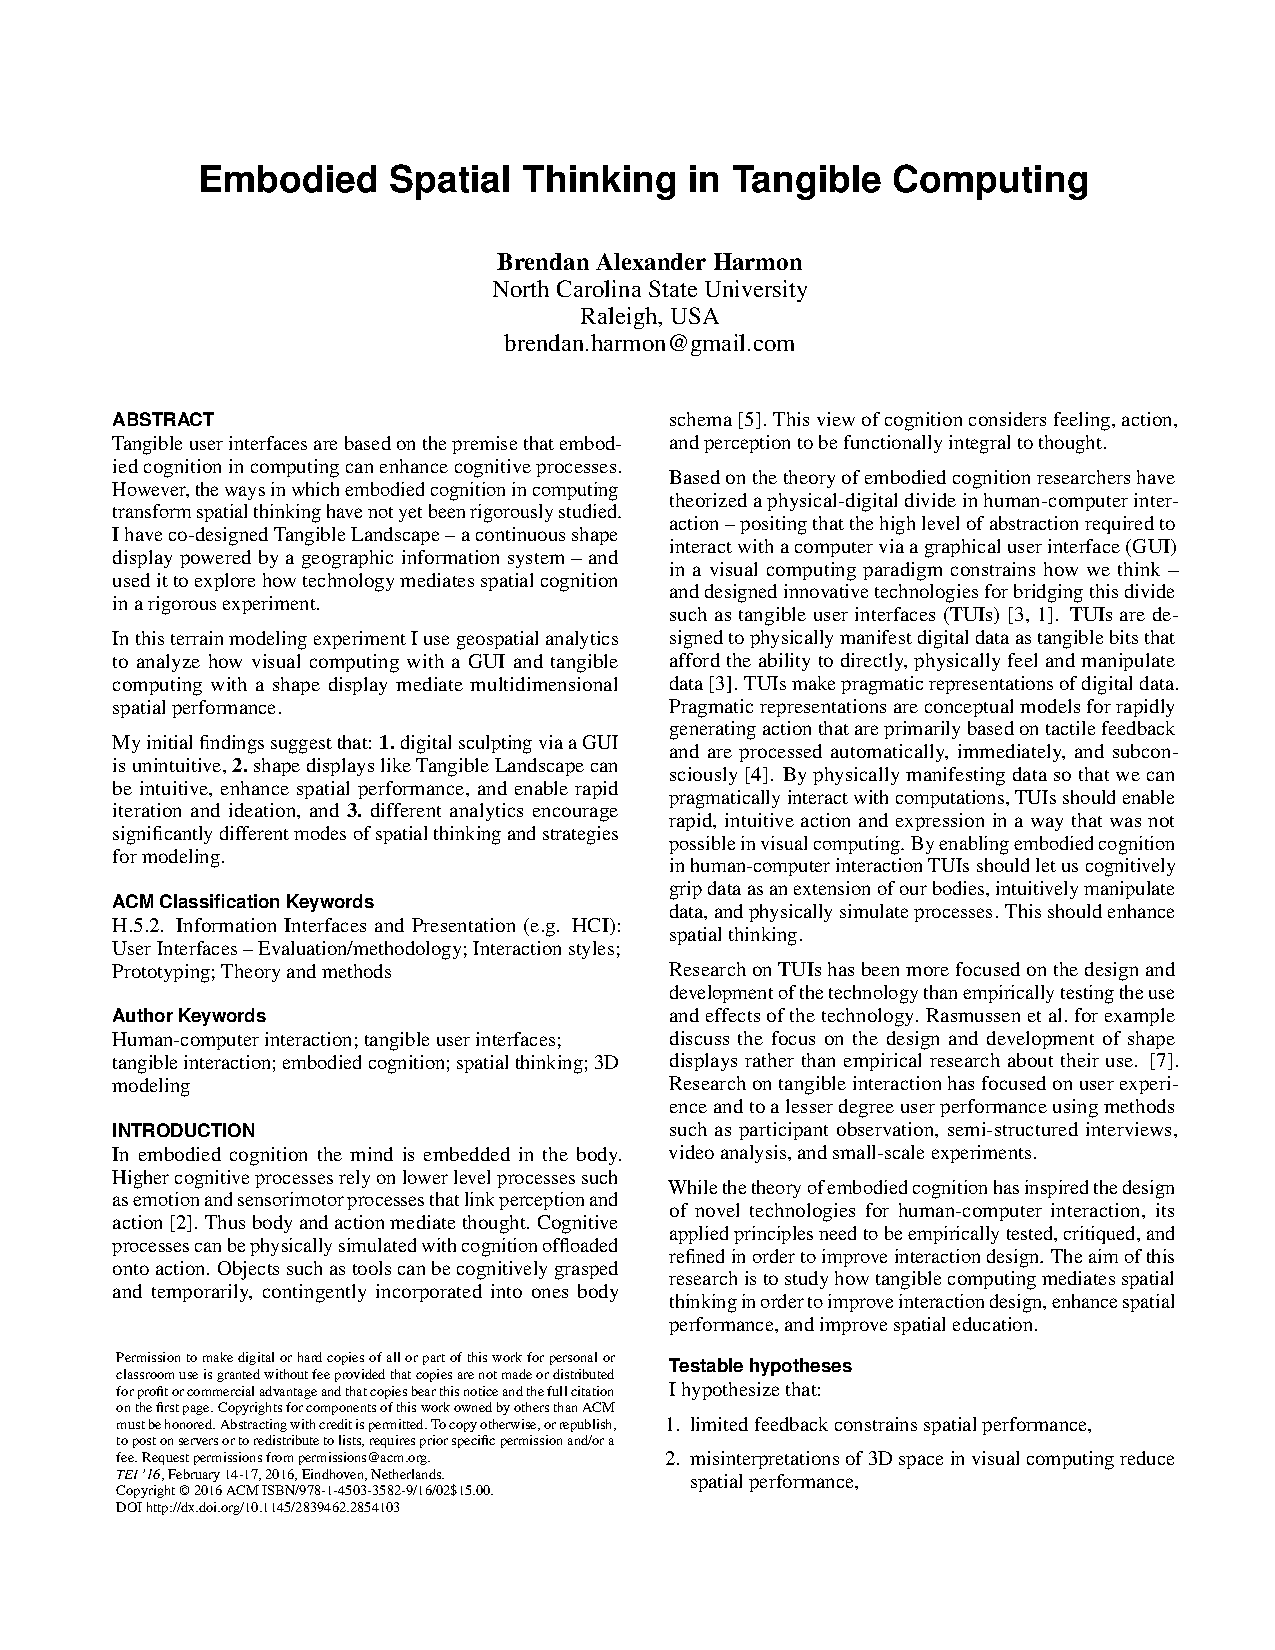
\includepdf[pages={-}]{tei_proceedings.pdf}
%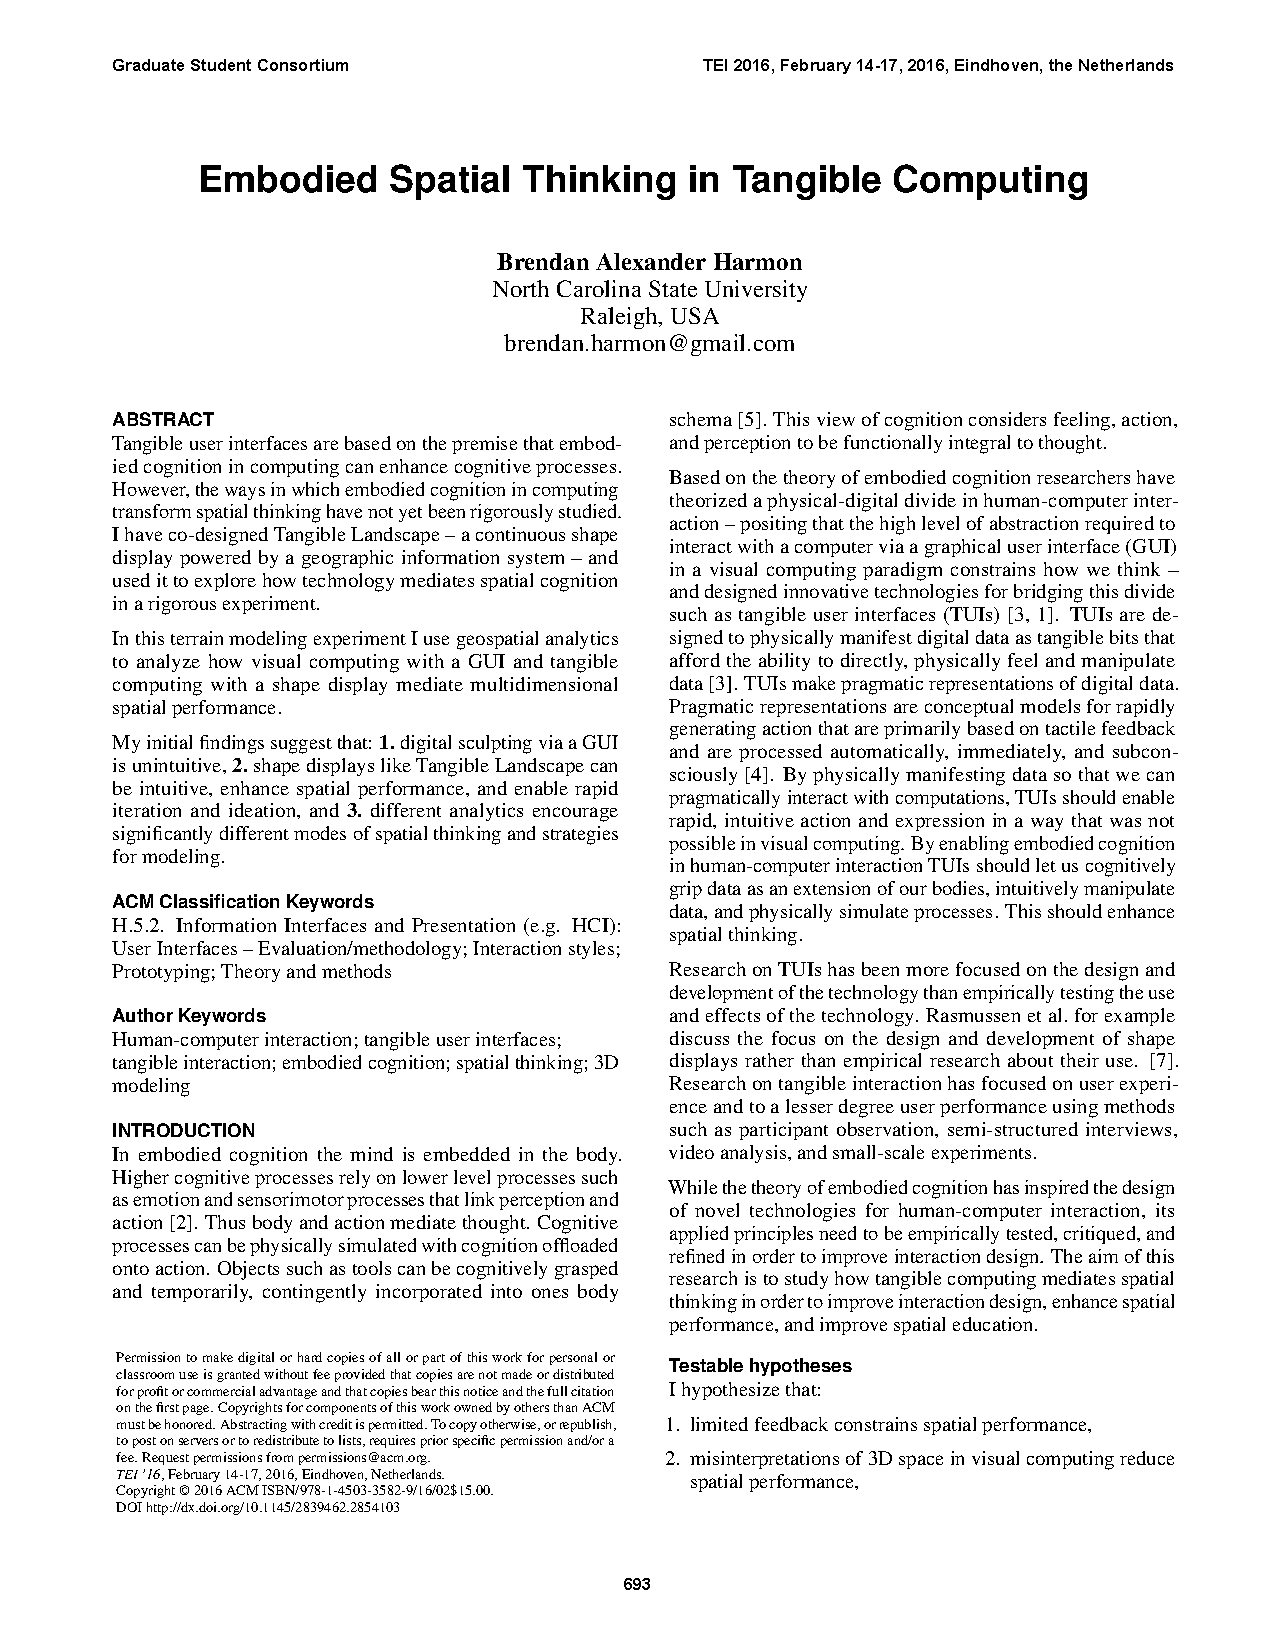
\includepdf[pages={-}]{p693-harmon.pdf}

% 

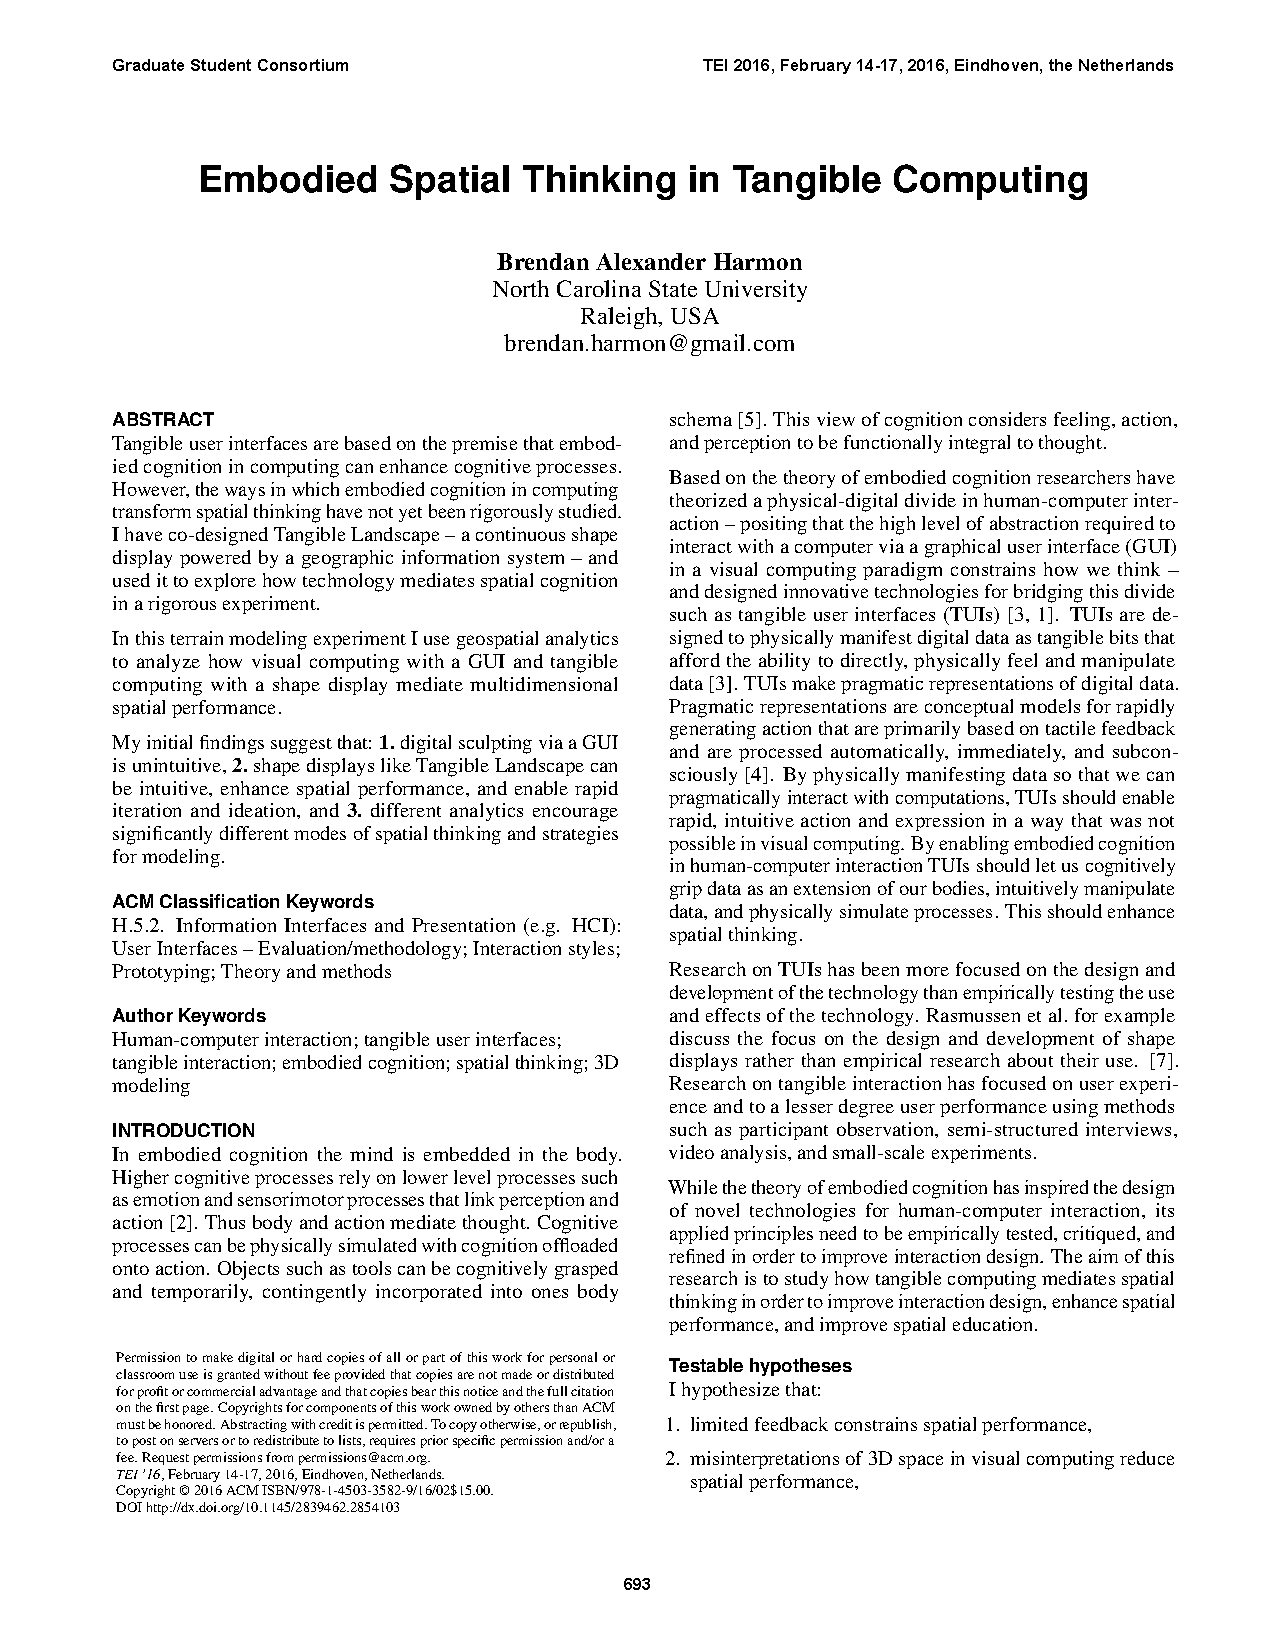
\includepdf[
pages={-},
scale={0.76},
offset={3mm 2mm},
%width=\textwidth,
%height=\textheight,
keepaspectratio,
noautoscale={true},
addtotoc={ % NOTE: changed section level from 1 to 6 to suppress section numbering
	1, section, 6, Introduction, tei-intro,
	2, section, 6, Methodology, tei-methods,
	2, section, 6, Preliminary Results, tei-results,
	3, section, 6, Future Work, tei-future,
	3, section, 6, Conclusions, tei-conc,
	3, section, 6, Acknowledgements, tei-ack,
	4, section, 6, References, tei-ref
	},
addtolist={
	3, figure, 3D sketching with Tangible Landscape, tei-fig-1,
	3, figure, Standard deviation of differences, tei-fig-2,
	4, figure, Reference model, tei-fig-3,
	4, figure, Model made with projection augmented modeling, tei-fig-4,
	4, figure, Model made with digital sculpting, tei-fig-5
	},
]{resources/p693-harmon.pdf} %{resources/tei_proceedings.pdf}

\chapter{Tangible Landscape: Cognitively Grasping the Flow of Water}
\label{chap-three}

\textbf{Reprint}

\textbf{Brendan A. Harmon}, Anna Petrasova, Vaclav Petras, Helena Mitasova, and Ross K. Meentemeyer. 2016. Tangible Landscape: cognitively grasping the flow of water. In \emph{The International Archives of the Photogrammetry, Remote Sensing and Spatial Information Sciences}. Prague: International Society of Photogrammetry and Remote Sensing. DOI:\url{http://dx.doi.org/10.5194/isprsarchives-XLI-B2-647-2016 647}

\textbf{Attribution}

% what I did
I co-designed Tangible Landscape,
designed and ran this experiment,
and wrote this paper.
%
% what my co-authors did
Anna Petrasova, Vaclav Petras, and Helena Mitasova
contributed to this research by
collaboratively designing Tangible Landscape,
running the experiment,
and editing the paper.
%
Ross Meentemeyer
contributed with advice, guidance, support, and editing.

\vfil
\pagebreak

%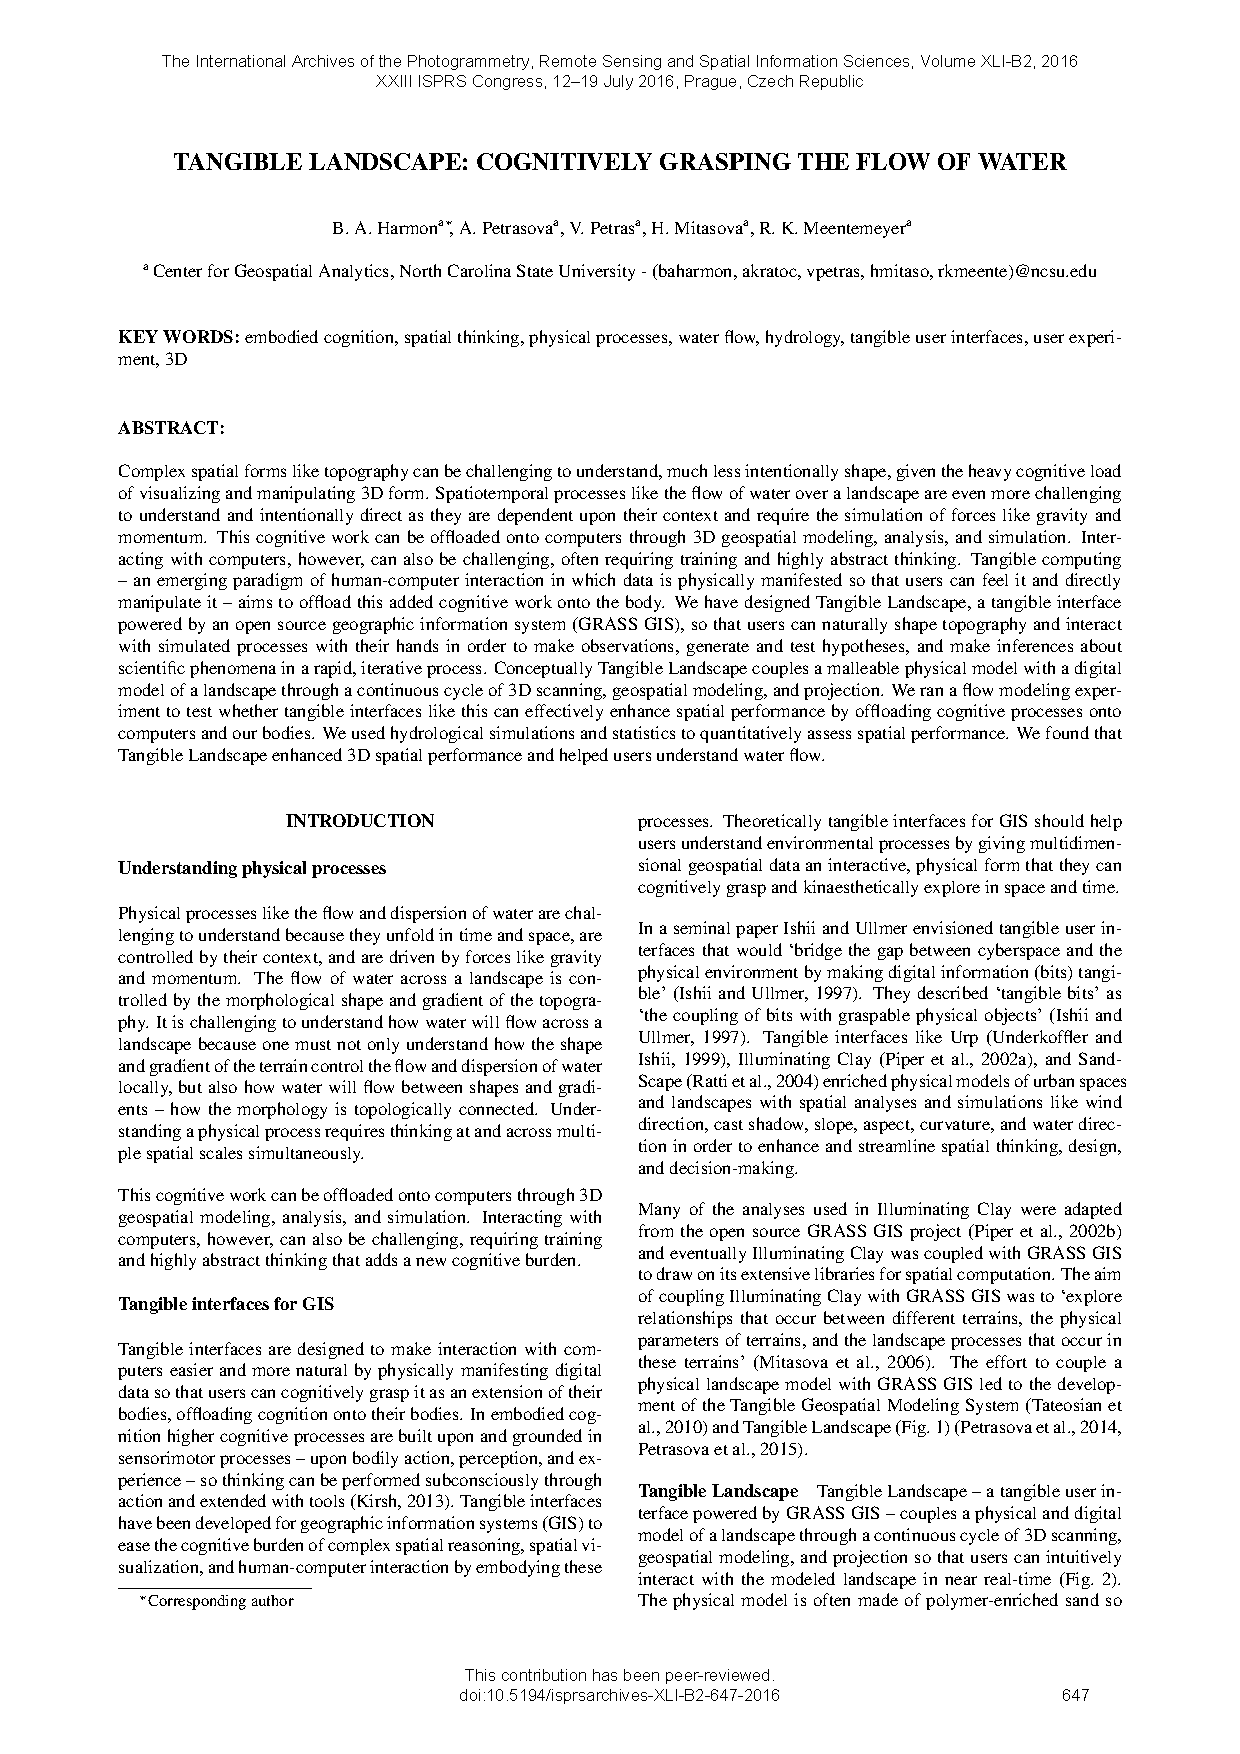
\includepdf[pages={-}]{isprs-archives-XLI-B2-647-2016.pdf}
%
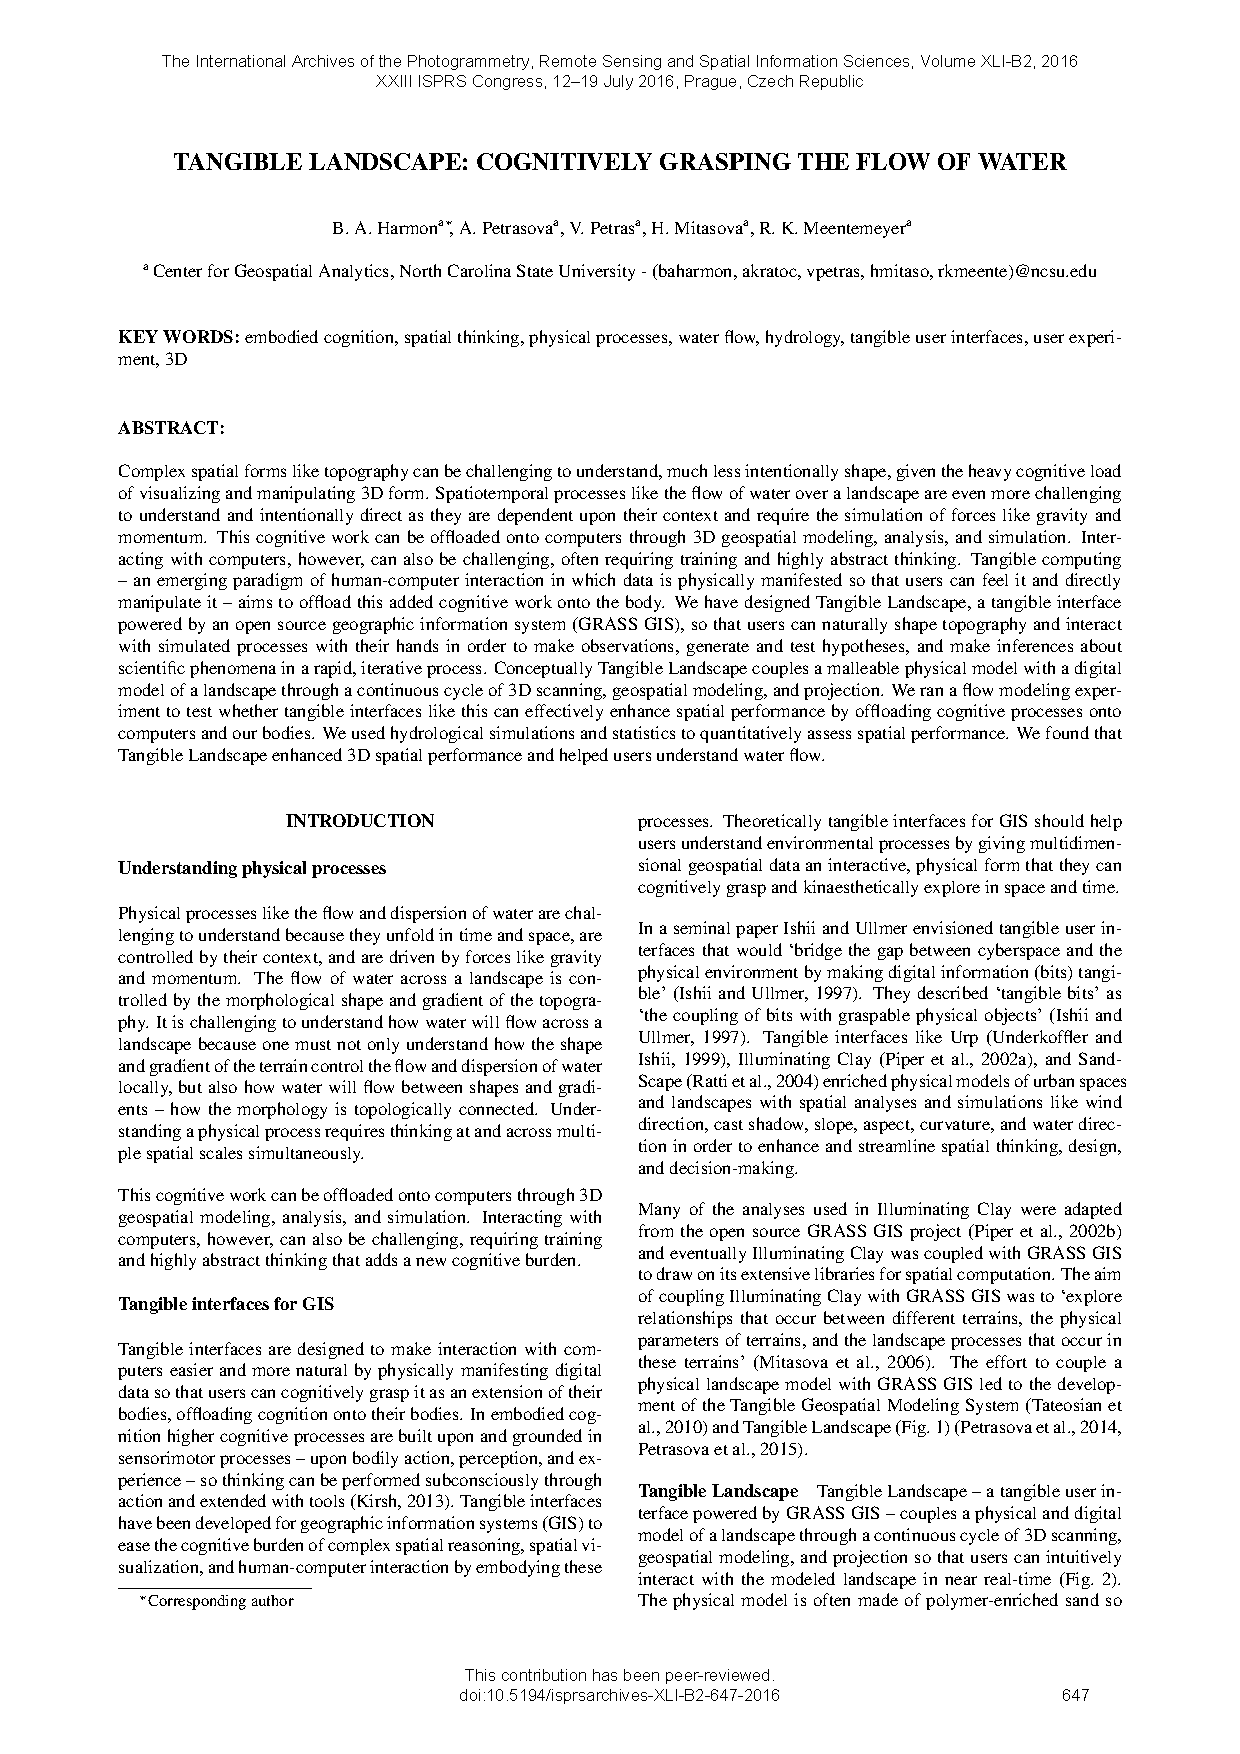
\includepdf[
pages={-},
scale={0.71},
offset={3mm 1mm},
%width=\textwidth,
%height=\textheight,
keepaspectratio,
noautoscale={true},
addtotoc={
	1, section, 6, Introduction, isprs-intro,
	2, section, 6, Methods, isprs-methods,
	4, section, 6, Results, isprs-results,
	4, section, 6, Discussion, isprs-discuss,
	5, section, 6, Conclusions, isprs-conc,
	5, section, 6, References, isprs-ref
	},
addtolist={
	2, figure, Modeling the flow of water with Tangible Landscape, isprs-fig-1,
	2, figure, How Tangible Landscape works, isprs-fig-2,
	2, figure, Reference landscape with simulated water flow, isprs-fig-3,
	3, figure, Digitally sculpting and tangibly sculpting, isprs-fig-4,
	4, table, Water depth statistics, isprs-tab-1,
	4, table, Minimum distance statistics, isprs-tab-2,
	4, table, Depression statistics, isprs-tab-3,
	4, table, Depression percentages, isprs-tab-4,
	6, figure, Water depth anlaysis, isprs-fig-5,
	6, figure, Depression analysis, isprs-fig-6,
	6, figure, Difference analysis, isprs-fig-7,
	6, figure, Detail of difference analysis, isprs-fig-8,
	7, figure, Minimum distance for digital sculpting, isprs-fig-9,
	7, figure, Minimum distance for tangible sculpting, isprs-fig-10
	},
]{resources/isprs-archives-XLI-B2-647-2016.pdf} %{resources/isprs_2016.pdf}

\chapter{Cognitively Grasping Topography with Tangible Landscape}
\label{chap-four}

%Published in...

%\textbf{Reprint}

\textbf{Attribution}

% what I did
I co-designed Tangible Landscape,
designed and ran the experiments,
and wrote the paper.
%
% what my co-authors did
Anna Petrasova, Vaclav Petras, and Helena Mitasova
contributed to this research by
collaboratively designing Tangible Landscape,
running the experiment,
and editing the paper.
%
Ross Meentemeyer, Gene Bressler, and Art Rice
contributed with advice, guidance, support, and editing.

\vfil
\pagebreak

%\includepdf[pages={-}]{tangible_topography.pdf}
%
\includepdf[
pages={-},
scale={0.9},
offset={2mm -4mm},
%width=\textwidth,
%height=\textheight,
keepaspectratio,
noautoscale={true},
addtotoc={
	1, section, 6, Introduction, tt-intro,
	9, section, 6, Tangible Landscape, tt-tl,
	16, section, 6, Coupling Experiment, tt-coupling,
	30, section, 6, Difference Experiment, tt-diff,
	34, section, 6, Water Flow Experiment, tt-water,
	37, section, 6, Discussion, tt-disc,
	42, section, 6, Future Work, tt-future,
	44, section, 6, Conclusions, tt-conc,
	45, section, 6, Appendix A, tt-app-a,
	47, section, 6, Appendix B, tt-app-b,
	49, section, 6, Appendix C, tt-app-c,
	50, section, 6, Appendix D, tt-app-d,
	51, section, 6, Appendix E, tt-app-e,
	51, section, 6, Appendix F, tt-app-f,
	51, section, 6, Appendix G, tt-app-g,
	52, section, 6, References, tt-ref
	},
addtolist={
	2, figure, Modeling the flow of water with Tangible Landscape, tt-fig-1,
	7, table, Actuated pin table interfaces, tt-tab-1,
	7, table, Augmented architectural modeling interfaces, tt-tab-2,
	7, table, Augmented clay interfaces, tt-tab-3,
	8, table, Augmented sandbox interfaces, tt-tab-4,
	10, figure, How Tangible Landscape works, tt-fig-2,
	10, figure, Modes of interaction with Tangible Landscape, tt-fig-3,
	10, figure, Scanning arms and hands as topography, tt-fig-4, 
	11, figure, Naturally exploring subsurface soil moisture, tt-fig-5,
	11, figure, Collaborative 3D sketching with VR, tt-tab-5,
	13, figure, Software schema for Tangible Landscape, tt-fig-6,
	14, figure, Accuracy assessment, tt-fig-7,
	14, figure, Scanning accuracy, tt-tab-6,
	15, figure, Casting polymeric sand models with 3D printed molds, tt-fig-8,
	16, figure, Sculpting a terrain model using the difference analytic, tt-fig-9,
	17, figure, Trail planning with Tangible Landscape, tt-fig-10,
	17, figure, Testing coastal flood defences with Tangible Landscape, tt-fig-11,
	17, figure, Managing the simulated spread of termites, tt-fig-12,
	18, figure, Participants, tt-tab-8,
	20, figure, {Coupling experiment: digital modeling}, tt-fig-13,
	20, figure, {Coupling experiment: analog modeling by hand}, tt-fig-14,
	20, figure, {Coupling experiment: projection augmented modeling}, tt-fig-15,
	22, table, Bivariate scatterplots of elevation values, tt-tab-9,
	23, figure, {Landforms identified by r.geomorphon}, tt-fig-16,
	23, figure, {Pairwise comparison by category of participants}, tt-fig-17,
	24, table, {Coupling experiment: per-cell statistics and analyses}, tt-tab-10,
	25, table, {Students}, tt-tab-11,
	25, table, {Academics and professionals}, tt-tab-12,
	26, table, {Landscape architecture students}, tt-tab-13,
	26, table, {GIS students}, tt-tab-14,
	27, table, {3D novices}, tt-tab-15,
	27, table, {3D experts}, tt-tab-16,
	28, table, {Coupling experiment: percent cells}, tt-tab-17,
	28, table, {Mean minimum distance}, tt-tab-18,
	32, table, Difference experiment, tt-tab-19,
	32, table, {Difference experiment: per-cell statistics}, tt-tab-20,
	32, table, {Difference experiment: geospatial analyses}, tt-tab-21,
	32, table, {Difference experiment: percent cells}, tt-tab-22,
	33, table, {Difference experiment: comparison}, tt-tab-23,
	34, figure, Water flow experiment, tt-fig-18,
	35, table, {Water flow experiment: per-cell statistics}, tt-tab-24,
	35, table, {Water flow experiment: geospatial analyses}, tt-tab-25,
	35, table, {Water flow experiment: percent cells}, tt-tab-26,
	36, table, {Water flow experiment: comparison}, tt-tab-27,
	38, table, {Interviews}, tt-tab-28,
	44, figure, {Tangible Landscape with robotic fabrication}, tt-fig-20,
	45, table, {How to build Tangible Landscape}, tt-tab-29,
	46, figure, {Stickers}, tt-fig-21,
	46, figure, {System setup}, tt-fig-22
	},
]{resources/tangible_topography.pdf}

\chapter{Tangible Modeling with Open Source GIS}
\label{chap-five}

\textbf{Reprint}

Petrasova, A., Harmon, B., Petras, V., \& Mitasova, H. (2015). Tangible Modeling with Open Source GIS. Springer International Publishing. \url{http://dx.doi.org/10.1007/978-3-319-25775-4}

\textbf{Attribution}

This book was a collaborative effort with my colleagues 
Anna Petrasova, Vaclav Petras, and Helena Mitasova.
I was the sole author of  chapter 1 and chapter 3. 
I co-authored chapter 7 and chapter 10 being responsible for approximately half of the content.
I also contributed extensively to the Appendix being responsible again for approximately half of the content.
My co-authors and I extensively edited the content, imagery, style, and structure of the entire book. 

\vfil
\pagebreak

%\includepdf[pages={-}]{tl_springer_book.pdf}

%\includepdf[pages={-}]{tl_book.pdf}


%
\includepdf[
pages={-},
%scale={0.75},
offset={0mm 1.75mm},
width=\textwidth,
height=\textheight,
keepaspectratio,
noautoscale={true},
addtotoc={
	11, section, 6, Introduction, intro,
	%23, subsection, 1, References, intro-ref,
	26, section, 6, System Configuration, sys-config,
	%39, subsection, 1, References, sys-config-ref,
	40, section, 6, Building Physical 3D Models, model-making,
	%60, subsection, 1, References, model-making-ref,
	61, section, 6, Basic Landscape Analysis, basic-analysis,
	%72, subsection, 1, References, basic-analysis-ref,
	73, section, 6, Surface Water Flow and Soil Erosion Modeling, water-flow-erosion,
	%84, subsection, 1, References, water-flow-erosion-ref,
	85, section, 6, Viewshed Analysis, viewshed,
	%90, subsection, 1, References, viewshed-ref,
	91, section, 6, Trail Planning, trails,
	%103, subsection, 1, References, trails-ref,
	104, section, 6, Solar Radiation Dynamics, solar,
	%110, subsection, 1, References, solar-ref,
	111, section, 6, Wildfire Spread Simulation, wildfire,
	%119, subsection, 1, References, wildfire-ref,
	120, section, 6, Coastal Modeling, coastal,
	%124, subsection, 1, References, coastal-ref,
	125, section, 6, Appendix A, app-a
	},
addtolist={
	13, figure, {Simulated water flow projected over a physical model}, book-fig-1,
	13, figure, {Physical, digital, and hybrid modeling processes}, book-fig-2,
	16, figure, {inFORM}, book-fig-3,
	19, figure, {The Tangible Geospatial Modeling System}, book-fig-4,
	20, figure, {3D sketching a dam with Tangible Landscape}, book-fig-5,
	21, figure, {Collaboratively sculpting a pond}, book-fig-6,
	22, figure, {3D sketching a levee breach}, book-fig-7,
	29, figure, {System configuration}, book-fig-8,
	30, figure, {Mobile system setup}, book-fig-9,
	31, figure, {Laboratory system setup}, book-fig-10,
	34, table, {Naming conventions for GRASS GIS modules}, book-tab-1,
	36, figure, {Mesh generated by Kinect Fusion}, book-fig-11,
	37, figure, {Calibration}, book-fig-12,
	41, figure, {A CNC routed model of Sonoma Valley, CA}, book-fig-13,
	42, figure, {Sculpting a polymeric sand model}, book-fig-14,
	45, figure, {A laser cut contour model}, book-fig-15,
	46, figure, {A CNC routed model of Jockey's Ridge, NC}, book-fig-16,
	47, figure, {A CNC router carving a terrain model}, book-fig-17,
	47, figure, {How to prepare MDF for CNC routing}, book-fig-18,
	48, table, {CNC settings: horizontal rough cut with MDF}, book-tab-2,
	48, table, {CNC settings: parallel finish cut with MDF}, book-tab-3,
	49, figure, {Magnetic markers}, book-fig-19,
	49, figure, {Modes of interaction using markers}, book-fig-20,
	50, figure, {Casting polymeric sand from 3D printed molds}, book-fig-21,
	51, figure, {Casting polymeric sand from CNC routed molds}, book-fig-22,
	51, figure, {A thermoformed polystyrene model}, book-fig-23,
	52, figure, {3D renderings of lidar data}, book-fig-24,
	64, figure, {3 x 3 neighborhood around an elevation value}, book-fig-25,
	65, figure, {Slope and aspect maps}, book-fig-26,
	65, figure, {Profile and tangential curvature}, book-fig-27,
	66, figure, {Landforms identified with geomorphons}, book-fig-28,
	66, figure, {Geomorphons}, book-fig-29,
	67, figure, {Lake Raleigh Woods}, book-fig-30,
	68, figure, {Basic workflow with DEM differencing}, book-fig-31,
	70, figure, {Slope and aspect of a scanned model}, book-fig-32,
	70, figure, {Profile and tangential curvature of a scanned model}, book-fig-33,
	72, figure, {Landform classification for a scanned model}, book-fig-34,
	78, figure, {Flow accumulation and watershed boundaries}, book-fig-35,
	79, figure, {Water depth computed with r.sim.water}, book-fig-36,
	80, figure, {Erosion and deposition for a scanned model}, book-fig-37,
	81, figure, {Lake Raleigh and it's surroundings}, book-fig-38,
	81, figure, {Lake Raleigh's current conditions and a new scenario}, book-fig-39,
	83, figure, {Flood simulation for current conditions}, book-fig-40,
	83, figure, {Flood simulation for new scenario}, book-fig-41,
	86, figure, {Line of sight analysis}, book-fig-42,
	87, figure, {Lake Raleigh Woods DSM}, book-fig-43,
	88, figure, {Placing a marker to identify a viewpoint}, book-fig-44,
	89, figure, {Viewsheds}, book-fig-45,
	90, figure, {Viewsheds from new buildings}, book-fig-46,
	94, figure, {The TSP applied to a network of potential trails}, book-fig-47,
	94, figure, {The slope and cross-slope of a trail}, book-fig-48,
	97, figure, {Friction map for Lake Raleigh}, book-fig-49,
	99, figure, {A trail around Lake Raleigh}, book-fig-50,
	101, figure, {Trail analytics with Tangible Landscape}, book-fig-51,
	102, figure, {Iteratively designing trails with Tangible Landscape}, book-fig-52,
	106, figure, {Different configurations of buildings}, book-fig-53,
	108, figure, {Shadows cast by different building configurations}, book-fig-54,
	109, figure, {Direct solar irradiation}, book-fig-55,
	110, figure, {Solar irradiation for different building configurations}, book-fig-56,
	112, table, {Classes of the Anderson fuel model}, book-tab-4,
	114, figure, {Orthophotograph and fuel map for Centennial Campus}, book-fig-57,
	116, figure, {The simulated spread of fire without intervention}, book-fig-58,
	117, figure, {Creating a firebreak with Tangible Landscape}, book-fig-59,
	118, figure, {The spread of fire after creating a firebreak}, book-fig-60,
	118, figure, {The spread of fire after creating another firebreak}, book-fig-61,
	121, figure, {Jockey's Ridge, Nags Head, NC}, book-fig-62,
	122, figure, {Simulated inundation for Jockey's Ridge}, book-fig-63,
	123, figure, {Designs for pavilions on Roanoke Island, NC}, book-fig-64,
	123, figure, {Siting pavilions with Tangible Landscape}, book-fig-65,
	124, figure, {Simulated water flow and erosion for the pavilions}, book-fig-66,
	126, figure, {Landforms in the High Tatras, Slovakia}, book-fig-67,
	126, figure, {The evolution of Oregon Inlet}, book-fig-68,
	127, figure, {Simulated storm surge for Rodanthe, NC}, book-fig-69,
	127, figure, {Land change for a watershed in Charlotte, NC}, book-fig-70,
	128, figure, {Reconstruction of a paleolake, Mongolia}, book-fig-71,
	129, figure, {Sand models of beaches and streams}, book-fig-72,
	130, figure, {Simulated breach of a coal ash pond}, book-fig-73,
	130, figure, {Generating time-series data}, book-fig-74,
	131, figure, {Interacting with disease and invasion models}, book-fig-75,
	132, figure, {Exploring subsurface soil moisture}, book-fig-76,
	135, figure, {Starting GRASS GIS}, book-fig-77,
	135, figure, {Displaying raster maps}, book-fig-78,
	136, figure, {Running GRASS GIS modules}, book-fig-79
	},
]{resources/tl_springer_book.pdf}

\restoregeometry

%%---------------------------------------------------------------------------%%
% Appendices
%\ensureoddstart
\restoregeometry
\appendix
\newgeometry{margin=1in,lmargin=1.25in,footskip=\chapterfootskip, includehead, includefoot}

\chapter[GIS-based environmental modeling with tangible interaction and dynamic visualization]{GIS-based environmental modeling with tangible interaction}
%and dynamic visualization
\label{app-a}

\textbf{Reprint}

Anna Petrasova, \textbf{Brendan A. Harmon}, Vaclav Petras, and Helena Mitasova. 2014. GIS-based environmental modeling with tangible interaction and dynamic visualization. In D. P. Ames \& N. Quinn, eds. \emph{Proceedings of the 7th International Congress on Environmental Modelling and Software}. San Diego, California, USA: International Environmental Modelling and Software Society.

\textbf{Attribution}

Anna Petrasova, the lead author, 
co-designed the \nth{1} generation Tangible Landscape,
developed the code, 
co-developed the case studies,
and wrote this paper.

I, Vaclav Petras, and Helena Mitasova
also co-designed the \nth{1} generation Tangible Landscape,
co-developed the case studies,
wrote part of the paper,
and edited the paper.

\vfil
\pagebreak

%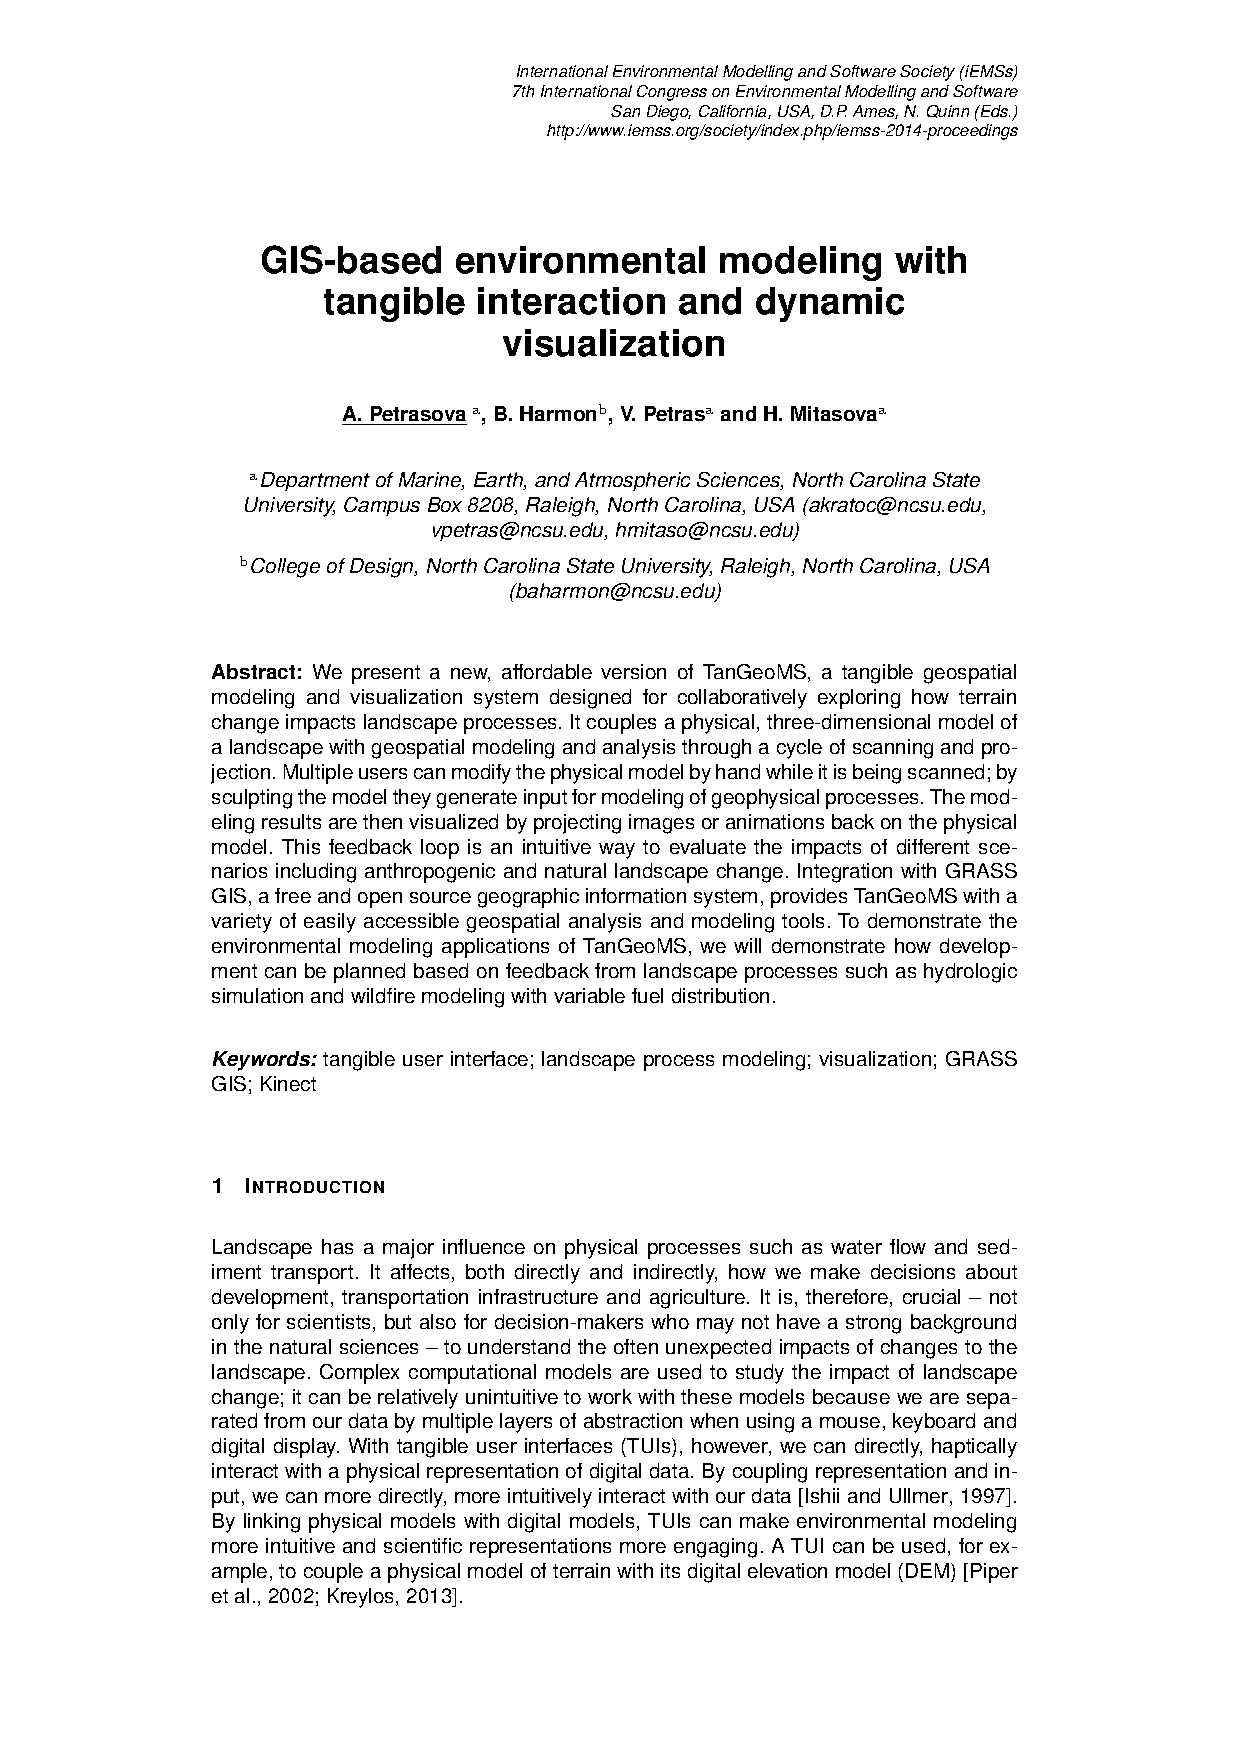
\includepdf[pages={-}]{gis-based-environmental.pdf}



%
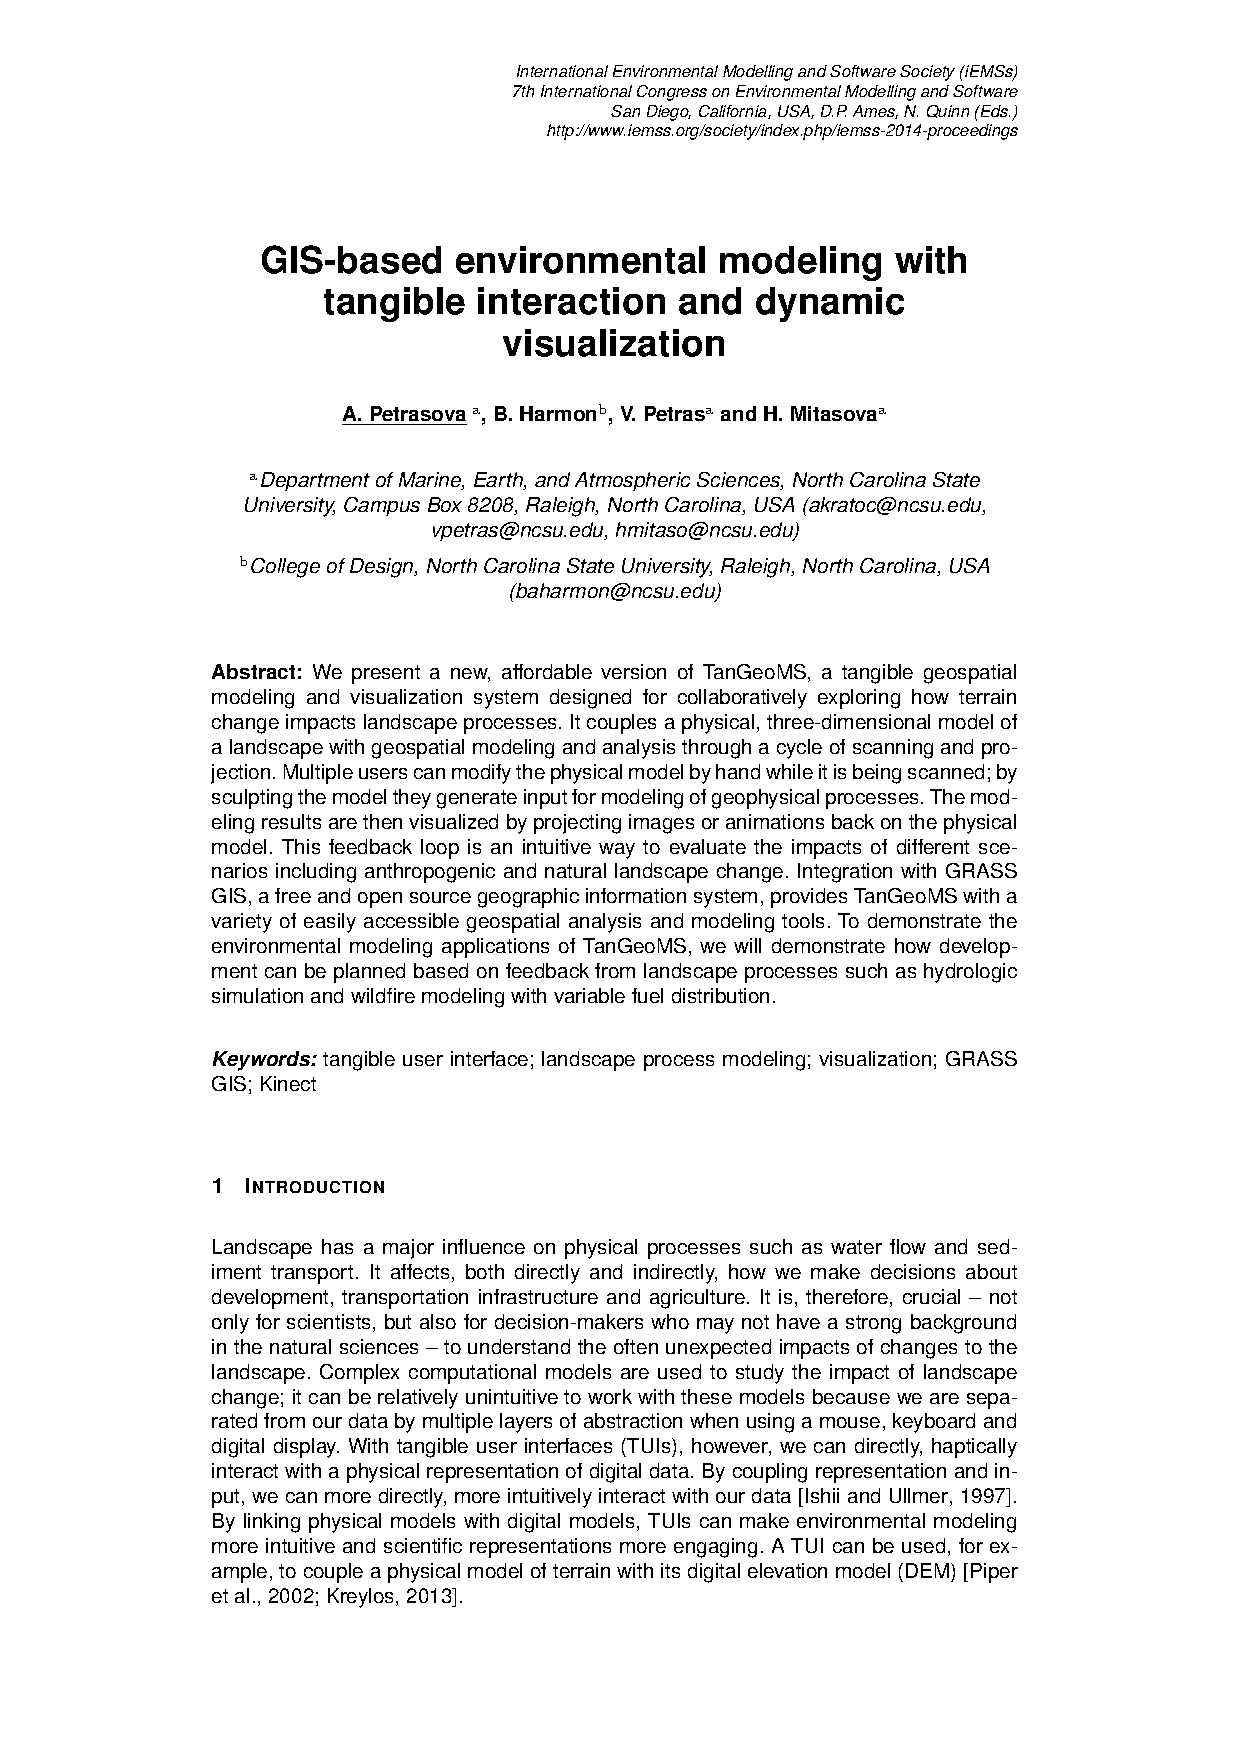
\includepdf[
pages={-},
scale={0.76},
offset={6mm -3mm},
%width=\textwidth,
%height=\textheight,
keepaspectratio,
noautoscale={true},
addtotoc={
	1, section, 6, Introduction, app-a-intro,
	2, section, 6, Methods, app-a-methods,
	5, section, 6, Applications, app-a-apps,
	7, section, 6, Discussion, app-a-discuss,
	8, section, 6, Conclusion, app-a-conc
	},
addtolist={
	2, figure, Physical setup, app-a-fig-1,
	3, figure, Different methods of creating models, app-a-fig-2,
	5, figure, Real-time water flow modeling, app-a-fig-3,
	6, figure, The current condition of Lake Raleigh Woods, app-a-fig-4,
	6, figure, First development scenario, app-a-fig-5,
	6, figure, First modified development scenario, app-a-fig-6,
	7, figure, Second development scenario, app-a-fig-7,
	7, figure, Wildfire spread simulation, app-a-fig-8
	},
]{resources/gis-based-environmental.pdf}

\chapter[Integrating Free and Open Source Solutions into Geospatial Science Education]
{Integrating FOSS into Geospatial Science Education}
\label{app-b}

\textbf{Reprint}

Vaclav Petras, Anna Petrasova, \textbf{Brendan Harmon}, Ross Meentemeyer, and Helena Mitasova. 2015. Integrating Free and Open Source Solutions into Geospatial Science Education. \emph{ISPRS Int. J. Geo-Information} 4, 2 (2015), 942–956. DOI:url{http://dx.doi.org/10.3390/ijgi4020942}

\textbf{Attribution}

Vaclav Petras and Anna Petrasova
developed this approach,
implemented methods 
for building course web pages,
and wrote this paper.

I developed and taught the course 
\emph{LAR582: GIS for Designers},
wrote the section about this course,
and edited the paper.

Ross Meentemeyer
directs the MGIST program at the Center for Geospatial Analytics at
North Carolina State University. 
He contributed to this paper with advice, guidance, support, and editing.

Helena Mitasova
pioneered this approach,
developed and taught the courses 
\emph{GIS/MEA582: Geospatial Modeling and Analysis} and
\emph{GIS595/MEA592: Multidimensional Geospatial Modeling},
wrote the sections about these courses,
and edited the paper.

\vfil
\pagebreak

%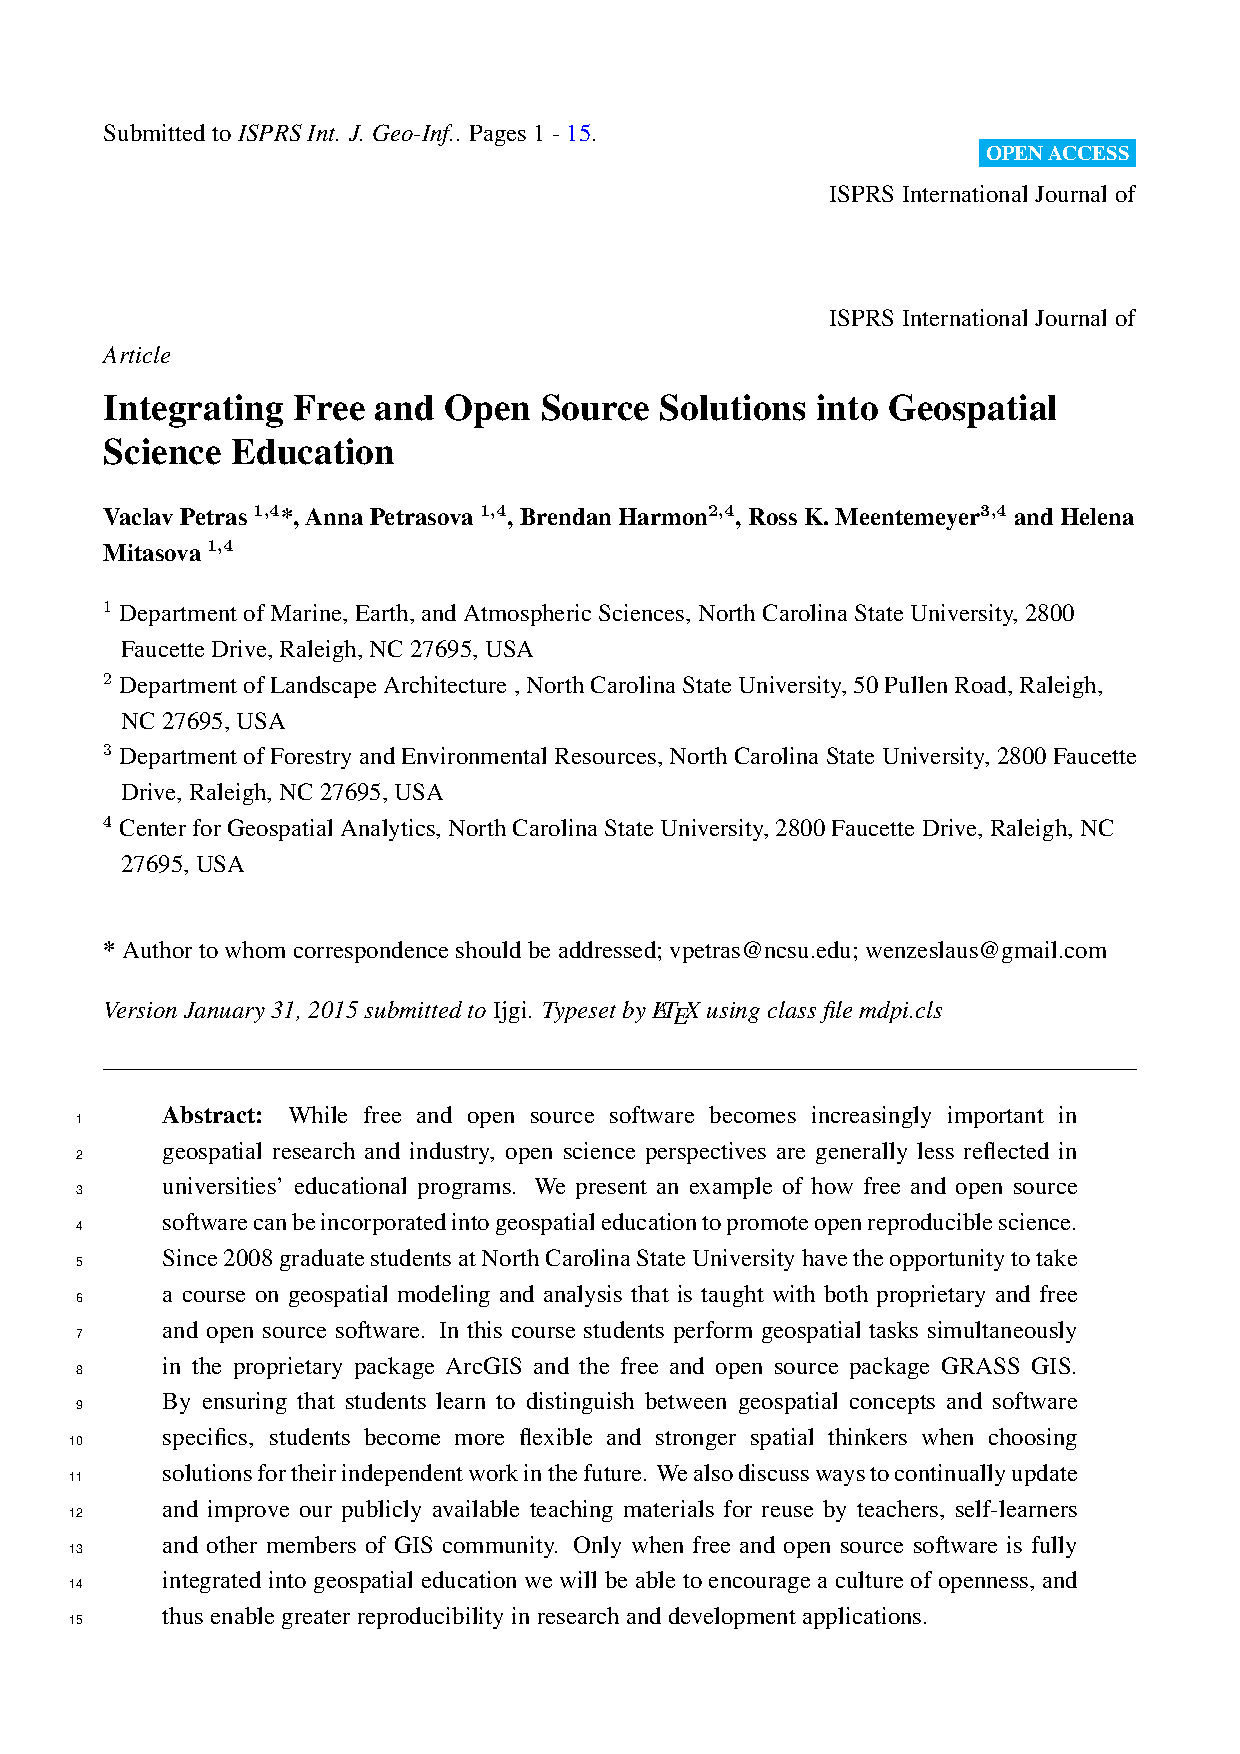
\includepdf[pages={-}]{integrating-free-open.pdf}



%
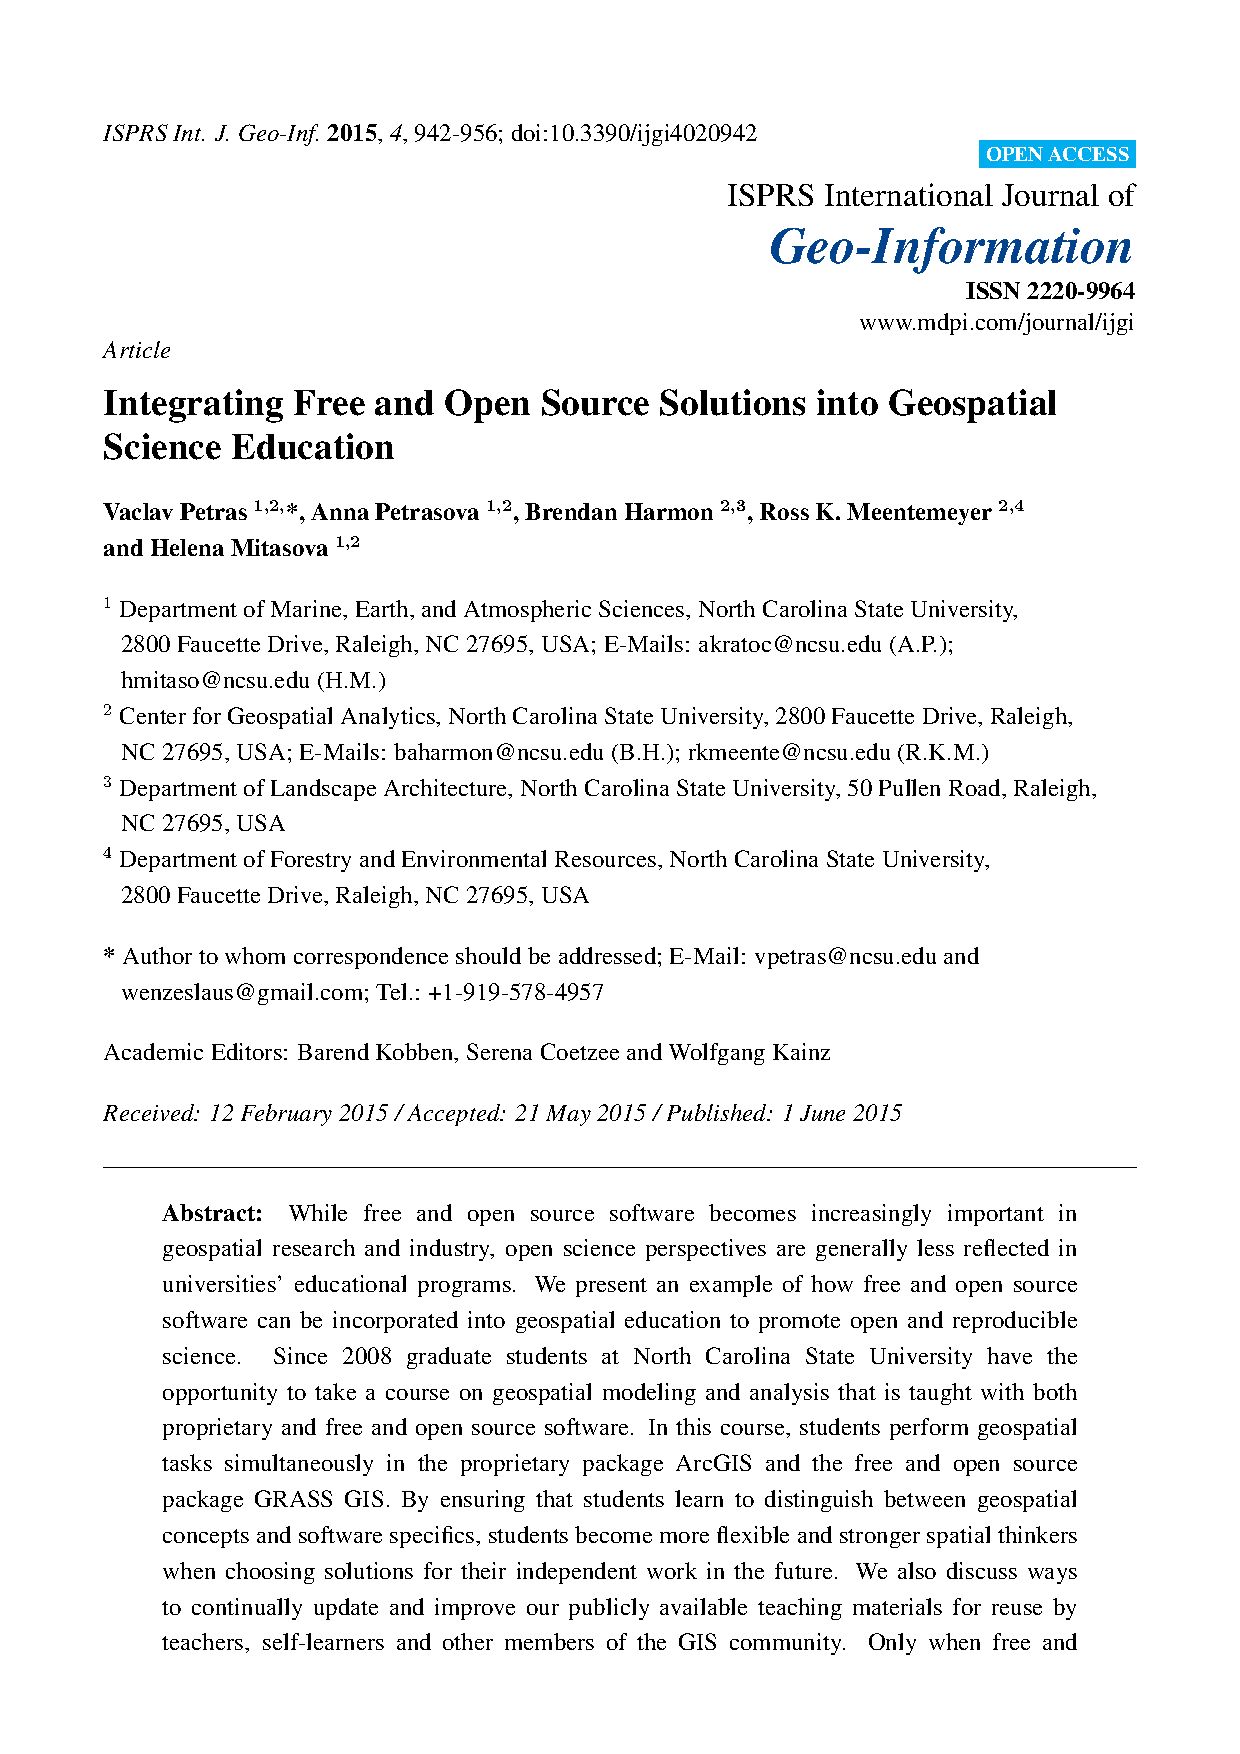
\includepdf[
pages={-},
scale={0.76},
offset={3mm 1mm},
%width=\textwidth,
%height=\textheight,
keepaspectratio,
noautoscale={true},
addtotoc={
	2, section, 6, Introduction, app-b-intro,
	3, section, 6, Approach to Course Design and Implementation, app-b-approach,
	7, section, 6, Course Implementation, app-b-imp,
	10, section, 6, Future Directions, app-b-future,
	11, section, 6, Conclusions, app-b-conc,
	12, section, 6, Appendix, app-b-app,
	14, section, 6, References, app-b-ref
	},
addtolist={
	4, figure, Instructions for the GRASS GIS part of an assignment, app-b-fig-1,
	6, figure, GIS GIS tutorial, app-b-fig-2,
	8, figure, Geospatial Modeling and Analysis assignment reports, app-b-fig-3,
	8, figure, Geospatial Modeling and Analysis exam and project paper, app-b-fig-4,
	9, figure, Students visualizing a digital elevation model, app-b-fig-5,
	10, figure, Students working on projects with Tangible Landscape, app-b-fig-6,
	10, figure, Students presenting designs for a trail system, app-b-fig-7
	},
]{resources/ijgi-04-00942.pdf}

\chapter{Open source approach to urban growth simulation}
\label{app-c}

\textbf{Reprint}

Anna Petrasova, Vaclav Petras, Derek Van Berkel, \textbf{Brendan A. Harmon}, Helena Mitasova, and Ross K. Meentemeyer. 2016. Open source approach to urban growth simulation. In \emph{The International Archives of the Photogrammetry, Remote Sensing and Spatial Information Sciences}. Prague: International Society of Photogrammetry and Remote Sensing. DOI:\url{http://dx.doi.org/10.5194/isprs-archives-XLI-B7-953-2016}

\textbf{Attribution}

Anna Petrasova, the lead author, 
developed the code, 
%designed the tangible interaction,
prepared the data and model parameters,
designed, implemented, and documented the case study, 
and wrote the paper.

Vaclav Petras helped to develop the code
and help to implement and document the case study.

Derek Van Berkel 
advised on the model,
helped to prepare the data and model parameters,
and edited the paper.

I helped document the case study
and edited the paper. 

%I co-designed the tangible interaction,
%digitally fabricated the physical model,
%helped to design, implement, and document the case study,
%and edited the paper.

Helena Mitasova and Ross Meentemeyer
advised on the concept and model
and edited the paper.

\vfil
\pagebreak

%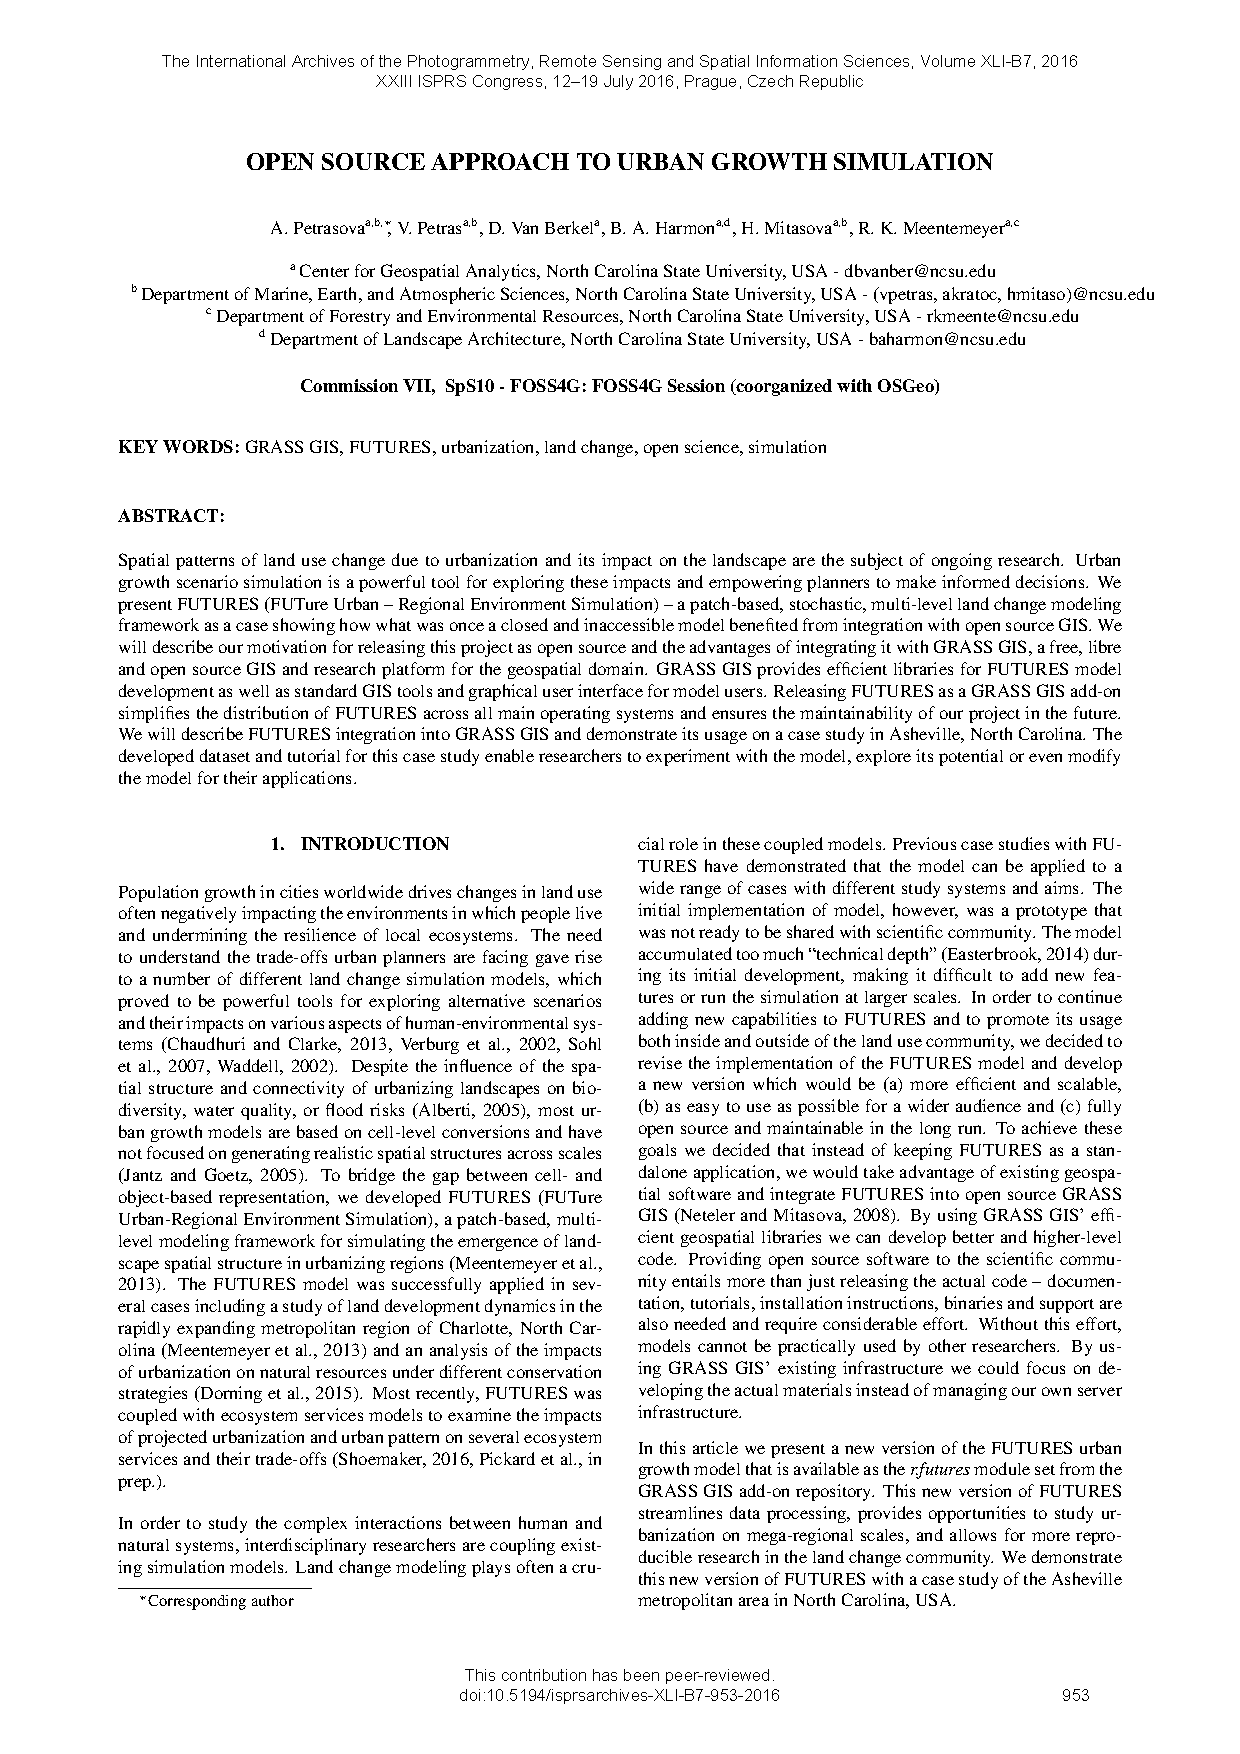
\includepdf[pages={-}]{isprs-archives-XLI-B7-953-2016.pdf}



%
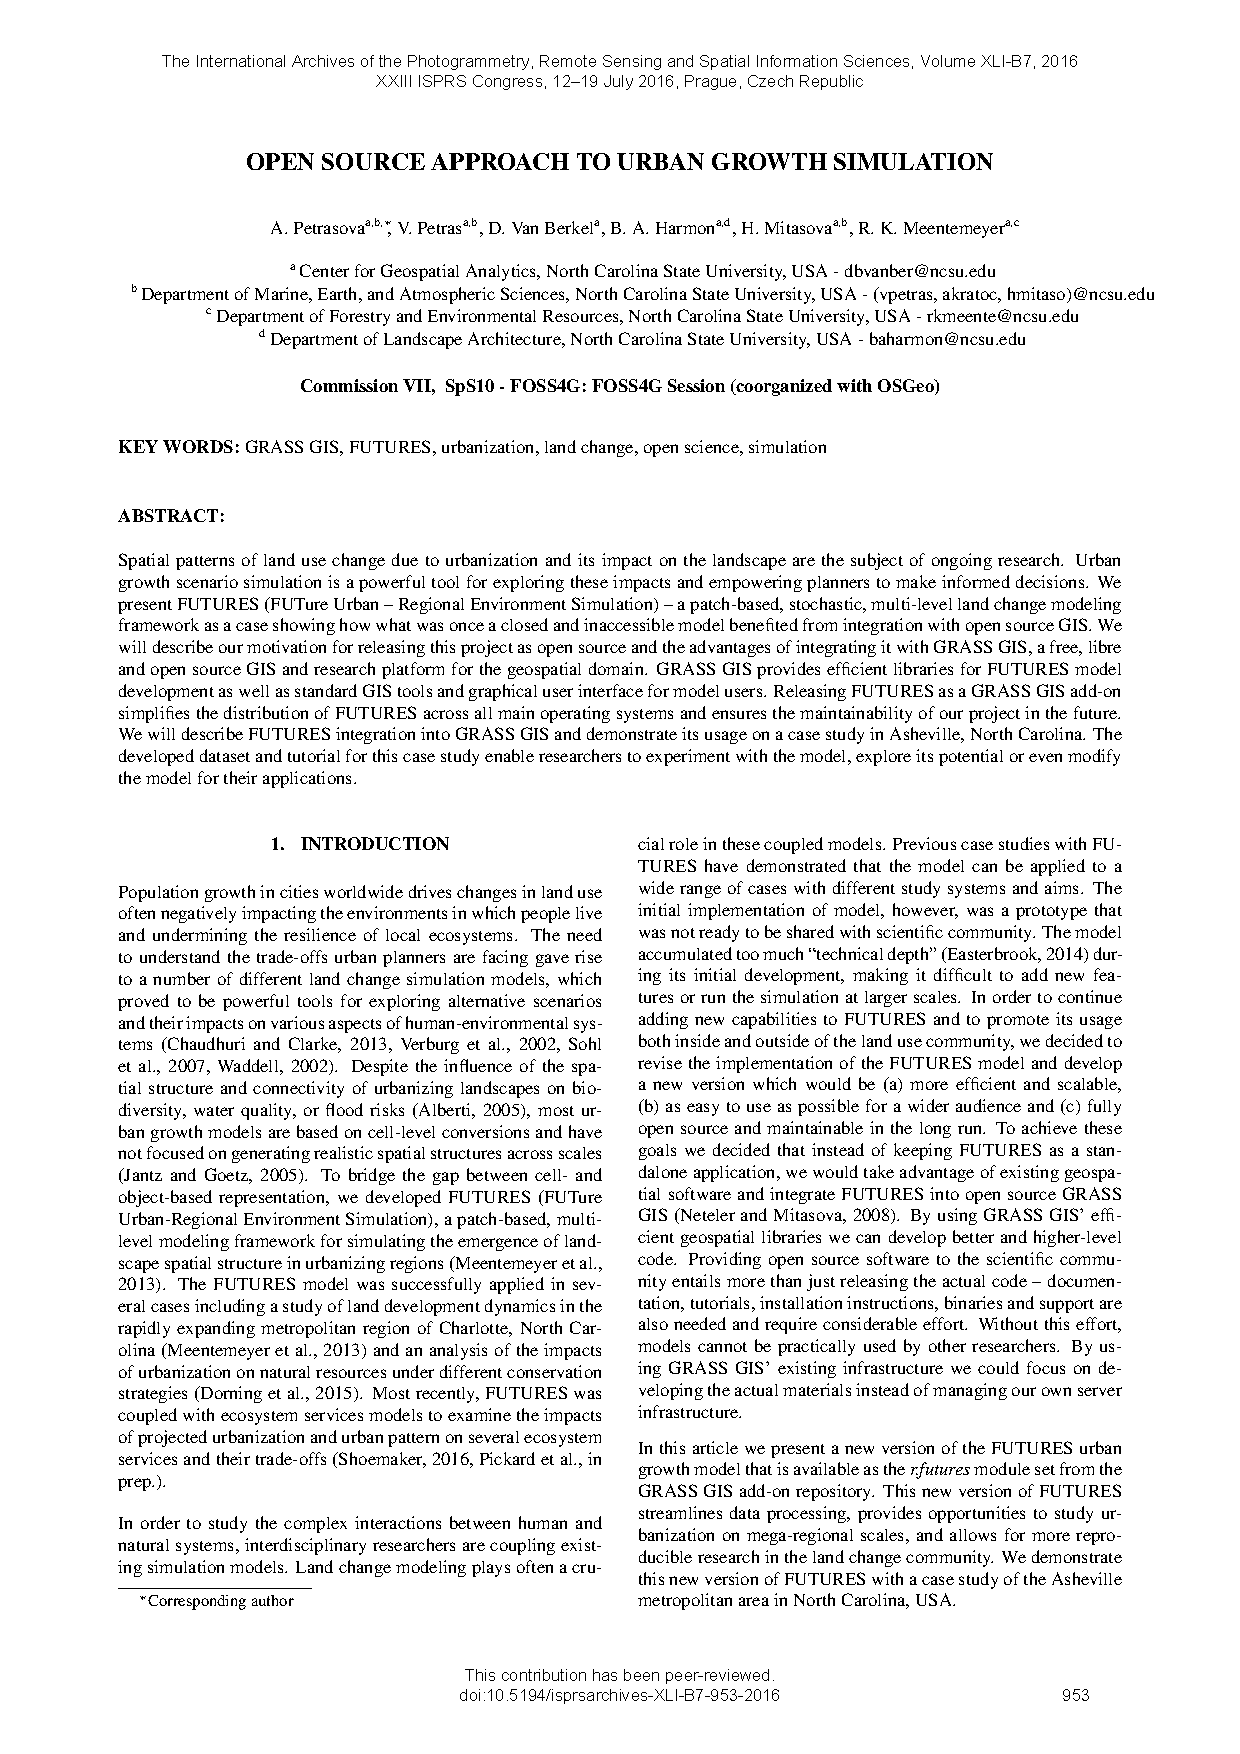
\includepdf[
pages={-},
scale={0.71},
offset={3mm 1mm},
%width=\textwidth,
%height=\textheight,
keepaspectratio,
noautoscale={true},
addtotoc={
	1, section, 6, Introduction, app-c-intro,
	2, section, 6,FUTURES Model, app-c-model,
	2, section, 6, Integration in GRASS GIS, app-c-integration,
	4, section, 6, Case Study, app-c-case,
	6, section, 6, Discussion, app-c-discuss,
	6, section, 6, Conclusion, app-c-conc,
	6, section, 6, References, app-c-ref
	},
addtolist={
	2, figure, Simplified schema of FUTURES conceptual model, app-c-fig-1,
	3, figure, Diagram of FUTURES workflow, app-c-fig-2,
	3, figure, An example of \emph{r.future.demand} output plot, app-c-fig-3,
	4, figure, {2011 land cover and protected areas in the Asheville, North Carolina}, app-c-fig-4,
	5, figure, Three realizations of multiple stochastic runs with different scenarios, app-c-fig-5,
	5, table, Predictors and estimated coefficients for the site suitability model, app-c-tab-1,
	5, figure, Area in km2 of converted land for urban sprawl and infill scenarios, app-c-fig-6,
	6, table, Time and memory needed to run the simulations, app-c-tab-2
	},
]{resources/isprs-archives-XLI-B7-953-2016.pdf}

\chapter{Immersive Tangible Geospatial Modeling}
\label{app-d}

\textbf{Reprint}

Payam Tabrizian, Anna Petrasova, \textbf{Brendan Harmon}, Vaclav Petras, Helena Mitasova, and Ross Meentemeyer. 2016. Immersive Tangible Geospatial Modeling. In \emph{Proceedings of the 24th ACM SIGSPATIAL International Conference on Advances in Geographic Information Systems. GIS ’16}. San Francisco, CA, USA: ACM, 88:1--88:4. DOI:http://dx.doi.org/10.1145/2996913.2996950

\textbf{Attribution} 
 
Payam Tabrizian, the lead author, 
developed the concept,
developed the code, 
designed, implemented, and documented the case study,
and wrote the paper.

Anna Petrasova
developed part of the code, 
co-designed Tangible Landscape,
helped to design, implement, and document the case study, 
wrote part of the paper,
and edited the paper.

I co-designed Tangible Landscape,
helped design its integration with immersive virtual environments,
helped to design, implement, and document the case study,
wrote part of the paper,
and edited the paper.

Vaclav Petras co-designed Tangible Landscape,
helped to implement and document the case study,
and edited the paper.

Helena Mitasova and Ross Meentemeyer
contributed with advice, guidance, support, and editing.

\vfil
\pagebreak

%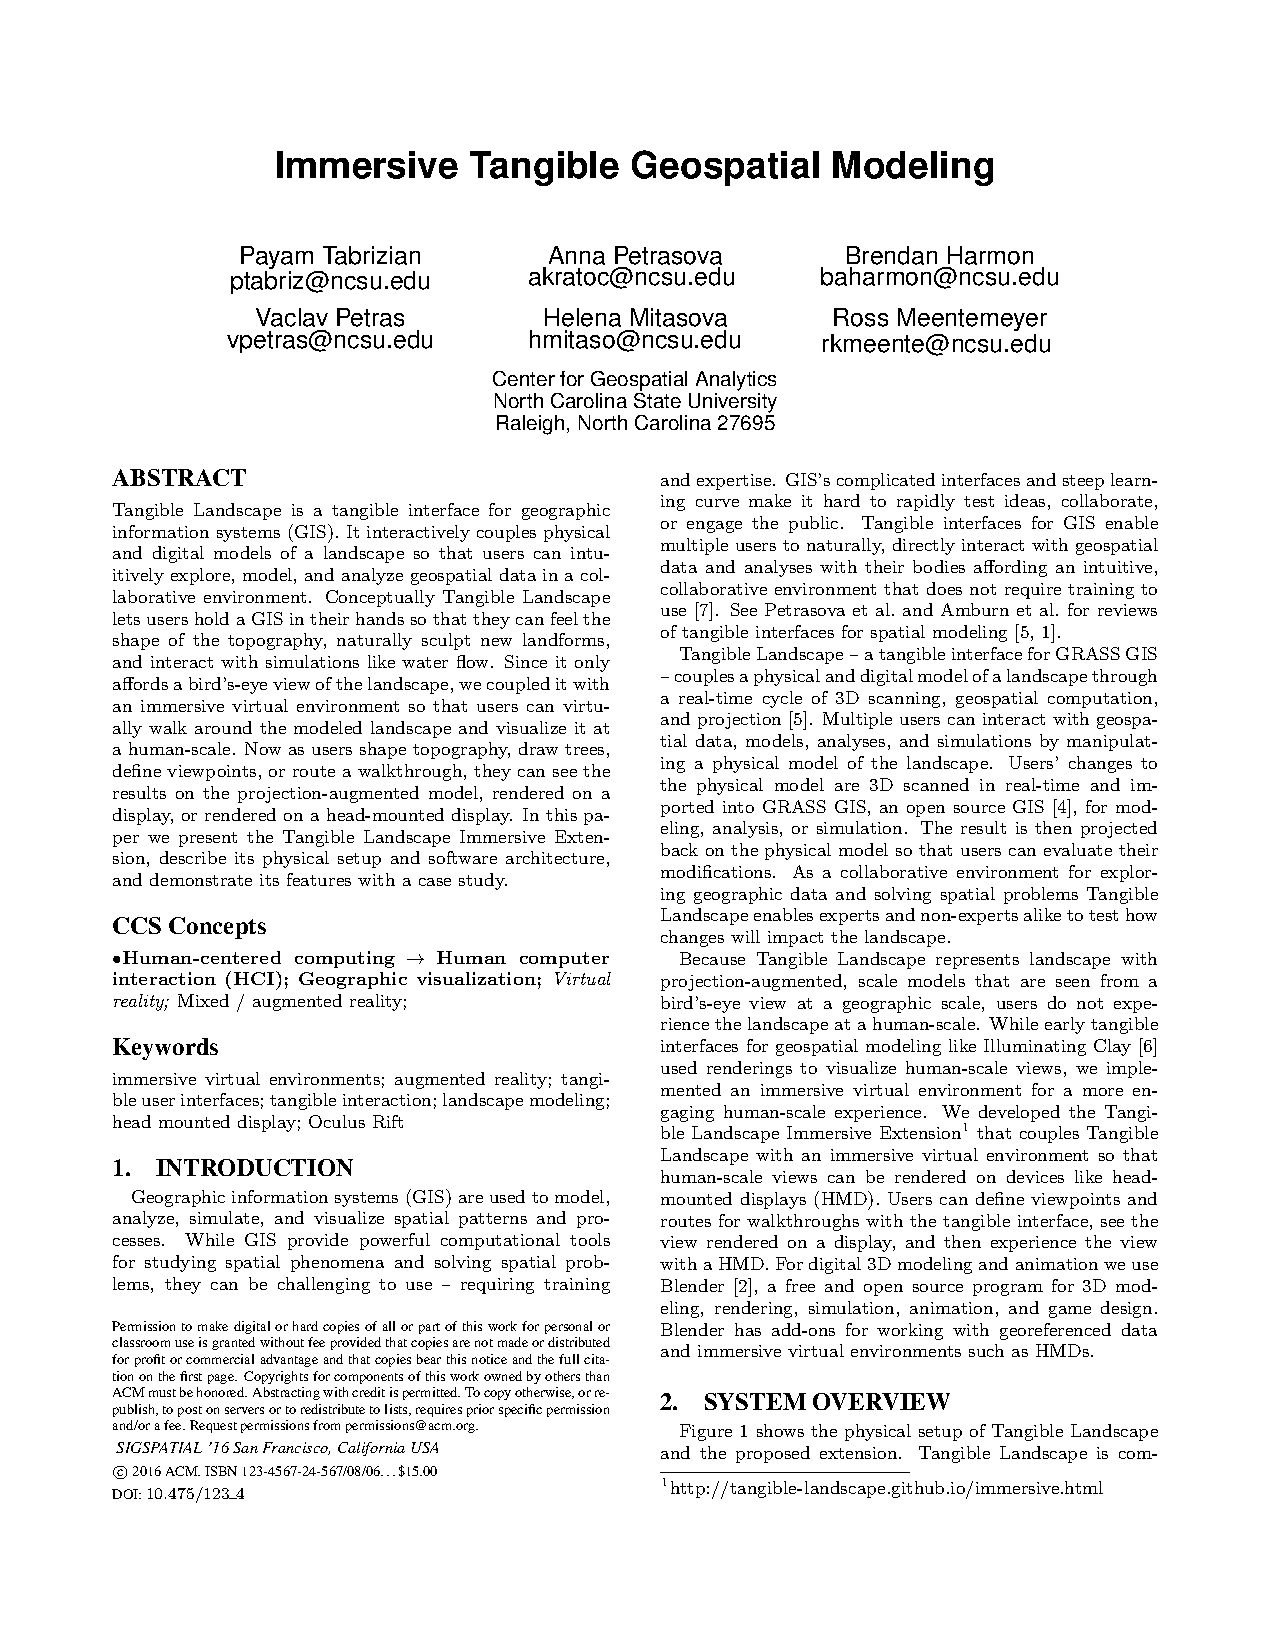
\includepdf[pages={-}]{immersive-tangible-geospatial.pdf}



%
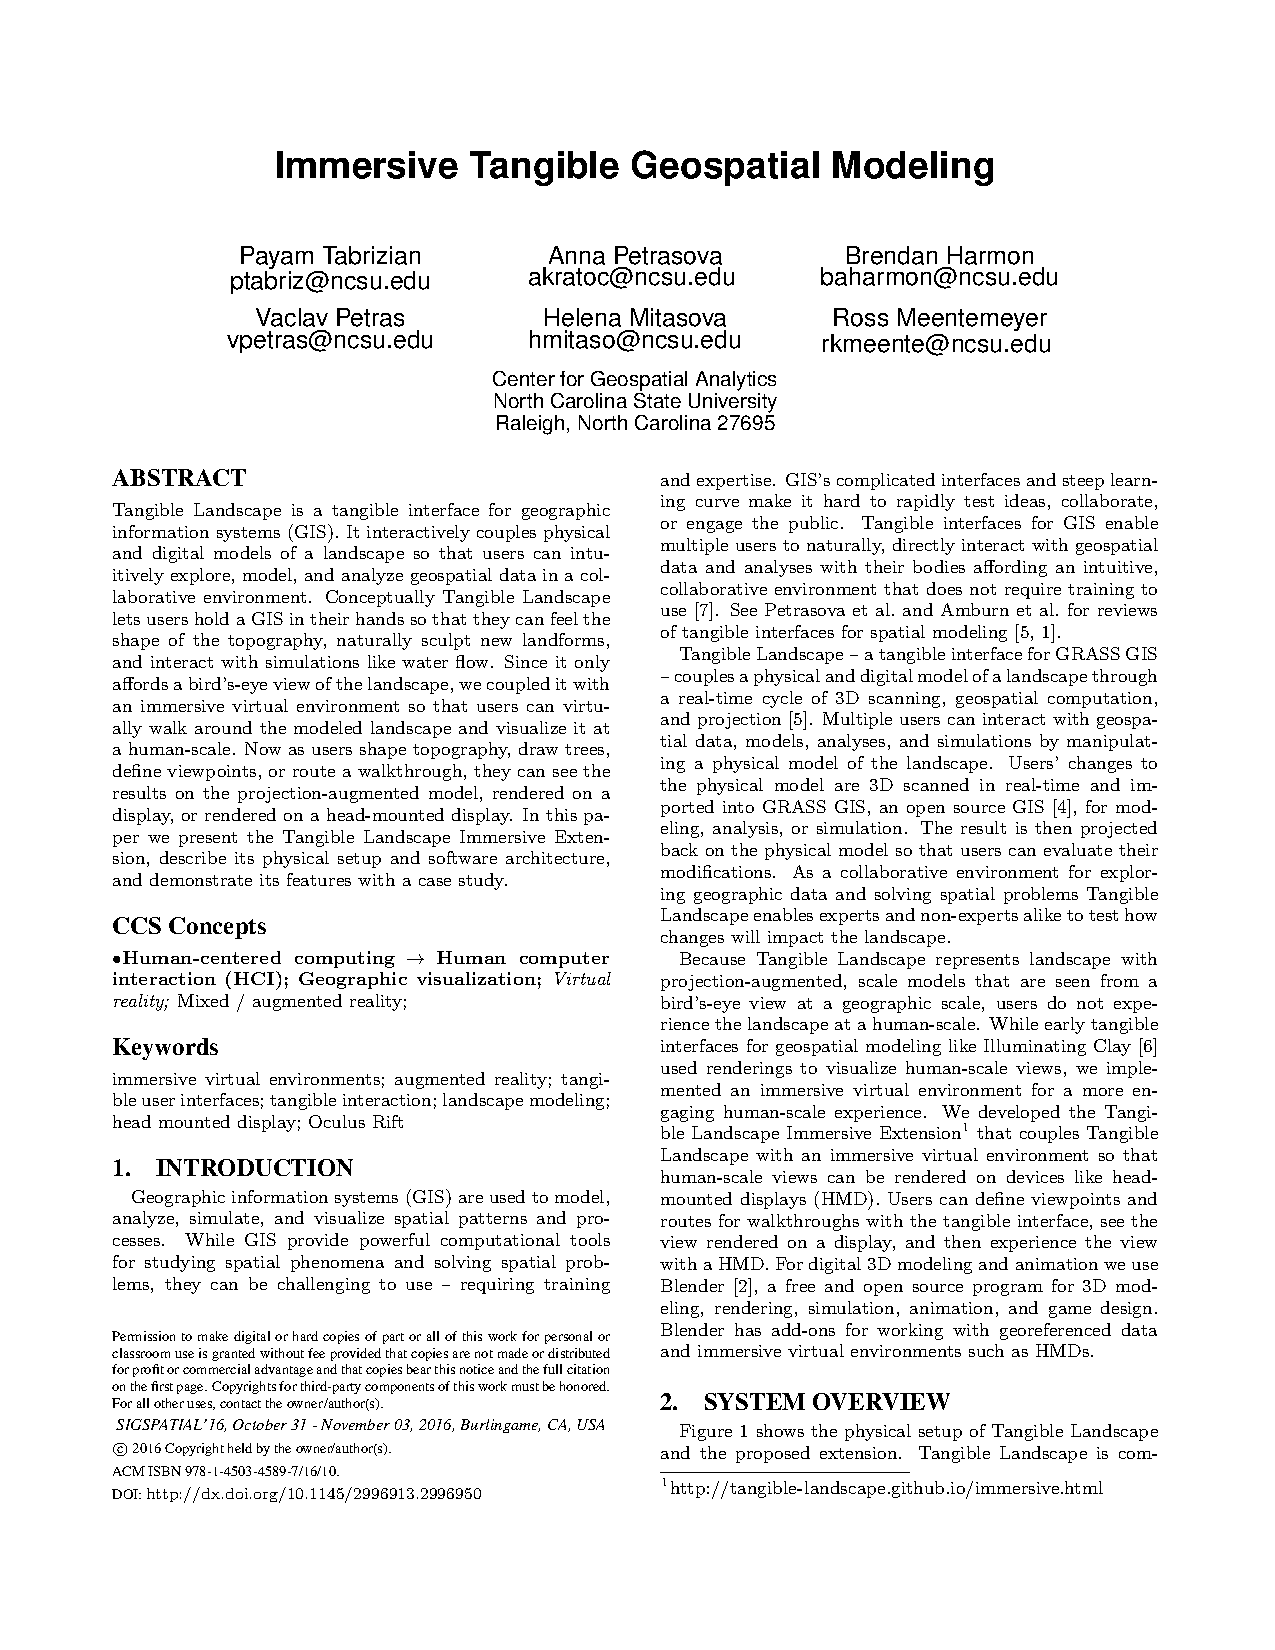
\includepdf[
pages={-},
scale={0.85},
offset={3mm 0mm},
%width=\textwidth,
%height=\textheight,
keepaspectratio,
noautoscale={true},
addtotoc={
	1, section, 6, Introduction, app-d-intro,
	1, section, 6,System Overview, app-d-sys,
	3, section, 6, Demonstration, app-d-demo,
	4, section, 6, Conclusion, app-d-conc,
	4, section, 6, References, app-d-ref
	},
addtolist={
	2, figure, Physical setup of Tangible Landscape and the proposed extension, app-d-fig-1,
	2, figure, Application process diagram, app-d-fig-2,
	2, figure, Interaction modes supported by Tangible Landscape, app-d-fig-3,
	3, figure, Sculpting topography to form ponds, app-d-fig-4,
	4, figure, Drawing patches of trees with a laser pointer, app-d-fig-5,
	4, figure, Designing an optimized trail, app-d-fig-6
	},
]{resources/a88-payam.pdf}

\chapter{Conference talks}
\label{app-e}

%\textbf{Attribution}

%I presented the following conference talks about Tangible Landscape:

Brendan A. Harmon, Helena Mitasova, and Anna Petrasova. 2014. Tangible geospatial modeling for landscape architects. In \emph{2014 Geodesign Summit}. Redlands, California: Esri.
\url{http://video.esri.com/watch/3170/tangible-geospatial-modeling-for-landscape-architects}

Brendan Harmon, Anna Petrasova, and Vaclav Petras. 2016. Serious gaming with Tangible Landscape. In \emph{Coffee \& Viz}. Raleigh, NC.
\url{https://baharmon.github.io/tei-2016/}

Brendan A. Harmon. 2016. Embodied spatial thinking in tangible computing. In \emph{TEI ’16: Tangible, Embedded, and Embodied Interaction 2016}. Eindhoven, Netherlands.
\url{http://ncsu-geoforall-lab.github.io/coffee-and-viz/hunt.html\#/9}

Brendan A. Harmon, Anna Petrasova, Vaclav Petras, Helena Mitasova, and Ross K. Meentemeyer. 2016. Creative spatial thinking with Tangible Landscape. In \emph{American Association of Geographers Annual Meeting 2016}. San Francisco, CA.
\url{http://baharmon.github.io/aag-2016/}

Brendan A. Harmon, Anna Petrasova, Vaclav Petras, Helena Mitasova, and Ross K. Meentemeyer. 2016. Tangible interaction for GIS. In \emph{FOSS4G NA 2016}. Raleigh, NC.
\url{http://baharmon.github.io/foss4g-na-2016/}

Brendan A. Harmon, Anna Petrasova, Vaclav Petras, Helena Mitasova, and Ross K. Meentemeyer. 2016. Tangible Landscape: cognitively grasping the flow of water. In \emph{International Society of Photogrammetry and Remote Sensing 2016}. Prague.
\url{https://baharmon.github.io/tangible-water-flow-presentation/}

Brendan A. Harmon, Anna Petrasova, Vaclav Petras, Helena Mitasova, and Ross K. Meentemeyer. 2016. Tangible geographies. In \emph{Royal Geographical Society Annual International Conference 2016}. London.
\url{https://baharmon.github.io/rgs-2016/}

% co-authored
%
%GIS-based modeling with tangible interaction
%Free and Open Source Software for Geospatial (FOSS4G) 2014
%\cite{Petrasova2014a}
%
%Using GRASS GIS through Python and tangible interfaces
%FOSS4G NA 2016
%\cite{Petrasova2016a}
%


\vfil
\pagebreak





\restoregeometry

%%---------------------------------------------------------------------------%%
%%  Bibliography 

%%  You can use the bibitem list.
%\bibliographystyle{unsrt}
%\begin{%thebibliography}{99}
%\bibitem{cb02}
%Casella, G. and Berger, R.L. (2002)
%\newblock {\it Statistical Inference, Second Edition.}
%Duxbury Press, Belmont, CA.
%
%\bibitem{t06}
%Tsiatis, A.A. (2006)
%\newblock {\it Semiparametric Theory and Missing Data.}
%Springer, New York.
%
%\end{thebibliography}

%% or use BibTeX
%\bibliographystyle{plain}
%\bibliography{baharmon-thesis.bib}
%\nociterec{*}

%\bibliographystyle{plainnat}%plainnat is necessary to enable the use of citet. Natbib style file.
%\ensureoddstart
\begin{spacing}{1}
 \setlength\bibitemsep{11pt} %22pt = 2*11pt, where fontsize is 11pt
 \addcontentsline{toc}{chapter}{{\uppercase{\bibname}}} %\textorpdfstring and \uppercase needed due to hyperref package http://www.latex-community.org/forum/viewtopic.php?f=44&t=16601
 %\vspace{-0.5in}
\titleformat{\chapter}[display]{\bf\filcenter
}{\chaptertitlename\ \thechapter}{11pt}{\bf\filcenter}
\titlespacing*{\chapter}{0pt}{-0.5in-9pt}{22pt}

%\nocite{*}
%\printbibliography[heading=myheading]
\end{spacing}
%\bibliographystyle{apalike}

%%---------------------------------------------------------------------------%%
%\ensureoddstart
\backmatter


\end{document}
